\documentclass[a4paper,twoside]{revtex4-1}
\usepackage[font=small,format=plain,labelfont=bf,up,textfont=it,up]{caption}
\usepackage[margin=2.5cm]{geometry} % change margin
\usepackage{subfigure}  %subfigures
\usepackage{graphicx}	%include graphics
\usepackage{fullpage}	
\usepackage{courier}     %\ttfamily
\usepackage{amsmath}	%Mathematics
\usepackage{mathtools} % "amsmath++"
\usepackage{amssymb}	%the R of real number, C of complex, etc.
\usepackage{float}		%To place figures where I want them
\usepackage{braket}		%The Quantum Mechanical Dirac notation: | > , < | , < > 
\usepackage{parskip}		
\usepackage[dvipsnames]{xcolor}		 %colored text
\usepackage{sidecap}		%Figure with a caption on the side
\usepackage{chngcntr}         %To adjust numbering of sections without having to use Chapters
\usepackage{nicefrac}


% Symbols used in model:
% Rate's (allways comes in handy)
\newcommand{\rate }[1]{\ensuremath{k_{\text{#1}}} }

%% Parameters: MFPT 
\newcommand{\lambdaS}{\ensuremath{\lambda_{\text{S}}  }}
\newcommand{\lambdaL}{\ensuremath{\lambda_{\text{L}}  }}
\newcommand{\gap}{\ensuremath{\delta_{\text{gap}}  }}

\newcommand{\weigthS}{\ensuremath{w_{\text{S}}}}
\newcommand{\LDNA}{\ensuremath{L_{\text{DNA}} }}


\newcommand{\Precap}{\ensuremath{P_{\text{RC}}}}
\newcommand{\Pub}{\ensuremath{P_{\text{ub}}}}
\newcommand{\PS}{\ensuremath{P_{\text{S}} }}
\newcommand{\PR}{\ensuremath{P_{\text{R}} }}
\newcommand{\ProbS}{\ensuremath{\rho_{\text{S}} }}
\newcommand{\ProbR}{\ensuremath{\rho_{\text{R}} }}
\newcommand{\NumberReturns}{\ensuremath{\overline{n}_{\text{return}}}}

%% Parameters: MonteCarlo simulation 
\newcommand{\Rmax}{\ensuremath{R_{\text{max}} }}
\newcommand{\Rprot}{\ensuremath{R_{\text{protein}} }}
\newcommand{\lambdaexcl}{\ensuremath{\lambda_\text{excl}} }


%% for the captions of the Supplemental Figures:
\newcommand{\figA}{\ensuremath{\textbf{(A)}}}
\newcommand{\figB}{\ensuremath{\textbf{(B)}}}
\newcommand{\figC}{\ensuremath{\textbf{(C)}}}
\newcommand{\figD}{\ensuremath{\textbf{(D)}}}

%% change style of section numbering
\renewcommand{\thesection}{\Alph{section}}
\renewcommand{\thesubsection}{\Roman{subsection}}

%% change the style of equation numbering 
\renewcommand{\theequation}{\arabic{equation}} 
%% suppress page numbering 
\pagenumbering{gobble}


\newcommand{\shuttletime}{\ensuremath{\Delta t_{\rm{shuttle}}}}
\newcommand{\tauBC}{\ensuremath{\Delta \tau_{\rm{BC}}}}
\newcommand{\tauCB}{\ensuremath{\Delta \tau_{\rm{CB}}}}


\newcommand{\singletargetdist}{\ensuremath{p_{\rm{bound}}}}
\newcommand{\shuttledist}{\ensuremath{P_{\rm{shuttle}}}}
\newcommand{\xPolT}{\ensuremath{x_{\rm{poly-T}}}}
\newcommand{\xTarget}{\ensuremath{x_{\rm{Target}}}}
\begin{document}
\begin{center}
{\bf \Large {update 10/10/2018}}
\end{center}


\section*{Before we start...}
Unfortunately, we cannot use Koen's results directly, because the files on the PNAS website were labelled incorrectly. In reality, the association data is taken using 1nM dCas9, while the dissociation (and occupation) data used 10nM dCas9. 
\\ \\
In essence, where Koen's project showed the data to be of 'class I' (see below), we will now show the data to really be of class II in stead. 
\\ \\ 
Moreover - as we will show in the end - Ilya's data dictates that the free-energy landscape drops between locations 9-12. Also, he has data using blocks of mismatches (pos 2-20, 3-20, 4-20, etc.) that indicates that the length of the mismatch block has little to no effect. 
We will show his data in the final section, but bare in mind that this has partially been our motivation to try different fits. 


\section{Two classes of fit results}
We get very similar on-target landscapes every time around. However, they are not as Koen got (not because of Koen, but because of PNAS!). \\
\\ 
For our interpretation we group the fit results based on the mismatch penalties. As you will see below, this changes 'what are the important stable states'. 
\\ \\ 
Another important concept we will speak of here is the 'aproximate' free-energy landscape of the on-target:
\begin{equation}
\Delta F_n = -\log \left( \sum_{i=0}^{n} e^{-E_i}\right)
\end{equation}
with $E_i = \sum_{j=o}^{i} \epsilon_C(j)$ representing the energy landscape as we have been talking about it so far. \\
Note that we thus construct this free-energy 'landscape' by combining systems in which everything is mismatched from position $n$ onwards. In this manner- with sufficient mismatch penalties - no state from $n$ onwards will have a significant contribution to the free-energy and you will be probing the on-target landscape. \\
As will be explained below, Ilya's measurements are essentially designed to return an estimate of this bound free-energy. 


\subsection{class I: non-constant $\epsilon_I$: Full R-loop still most stable state with multiple mismatches.}
 
\begin{itemize}
\item \textbf{Long story short: Took a while, but we realise this is actually not the relevant regime. You may just skip to next section.}
\item This is (more or less) the regime Koen's results are in.
\item With these values, even after placing a second mismatch the system's most stable state is when a complete R-loop has been formed. 
\item For as far as the dissociation experiment goes, any mismatched system can basically be seen to have two stable states: One with the completely formed R-loop and the other right before the mismatch.
\item Using some toy-modelling - not shown here as this eventually is not the important regime anyways - a good fit to both single and multiple mismatch dissociation rates - at the very least setting the ratio between the maximum values (see the fit) - nesseciates that $\epsilon_I \approx 1.5 k_BT$. 
\item However, in order to achieve suffiently low association rates and occupancies for PAM proximal mismatches, the $\epsilon_I$ needs to be larger. 
\item As a result, the fit basically used the on-target landscape only to set the overal stability (mostly) and essentially uses the mismatch penalties to create all contrasts between PAM distal and proximal mismatch configurations. 
\item Further fluctuations in the heatmaps exactly follow the pattern of the mismatch penalties. 
\item In this regime, placing more mismatches will decrease the association rate and occupancy, and increase the dissociation rate. 
\item Not yet a good fit to the single-mismatch association data
\item This is surely inconsistent with Ilya's data. Given the system still has stable states after multiple mismatches, it clearly matters how many will be placed for the effective association and dissociation rates (see the figure with blocks of mismatches in final section). 
\item Also the resulting free-energy landscape for the cognate site does not match that of Ilya's.
\end{itemize}


\begin{figure}[H]
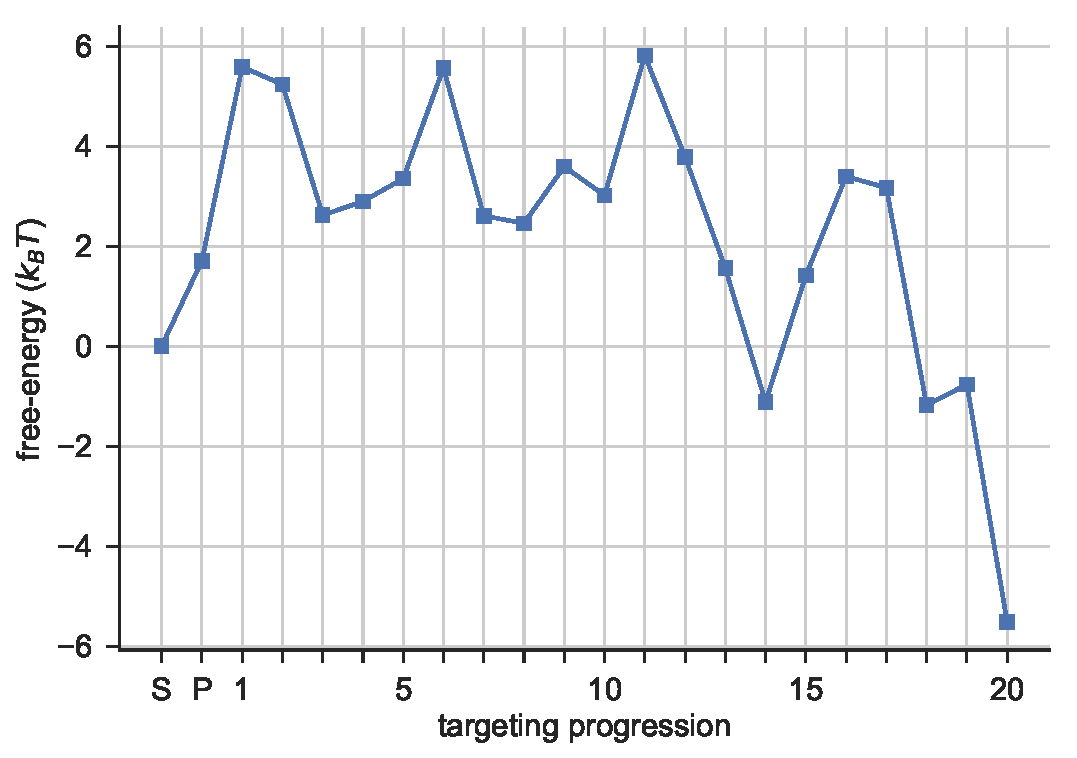
\includegraphics[scale=0.5]{fig23_10_10_2018.pdf}
\end{figure}

\begin{figure}[H]
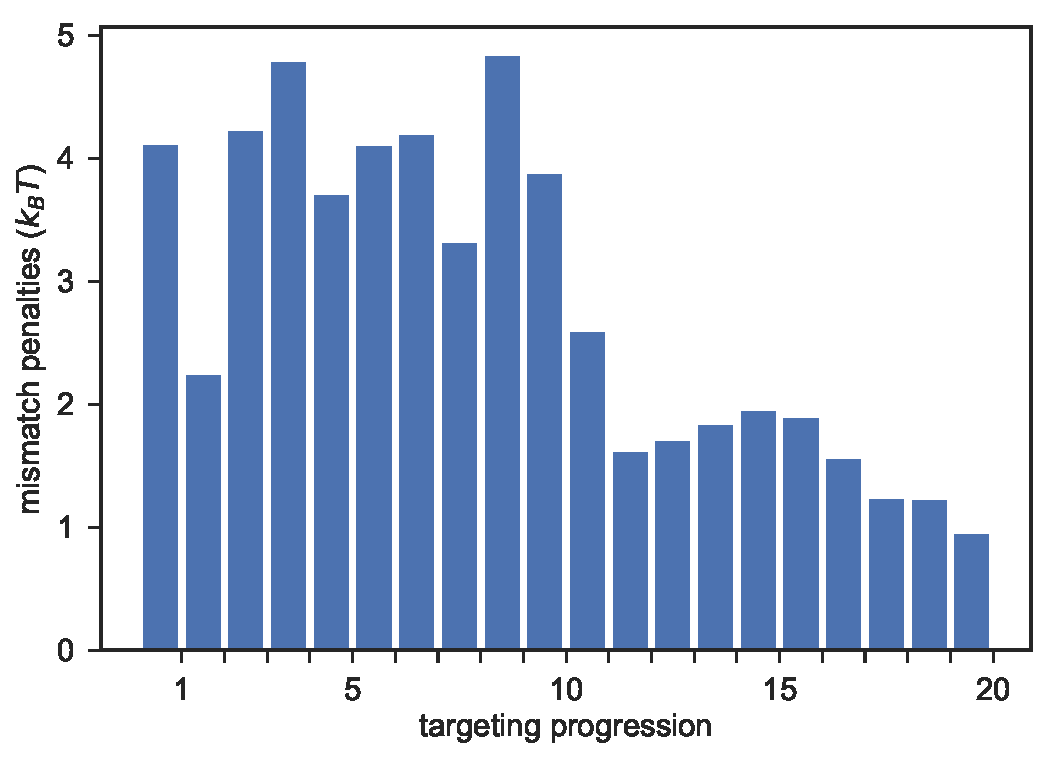
\includegraphics[scale=0.5]{fig24_10_10_2018.pdf}
\end{figure}

\begin{figure}[H]
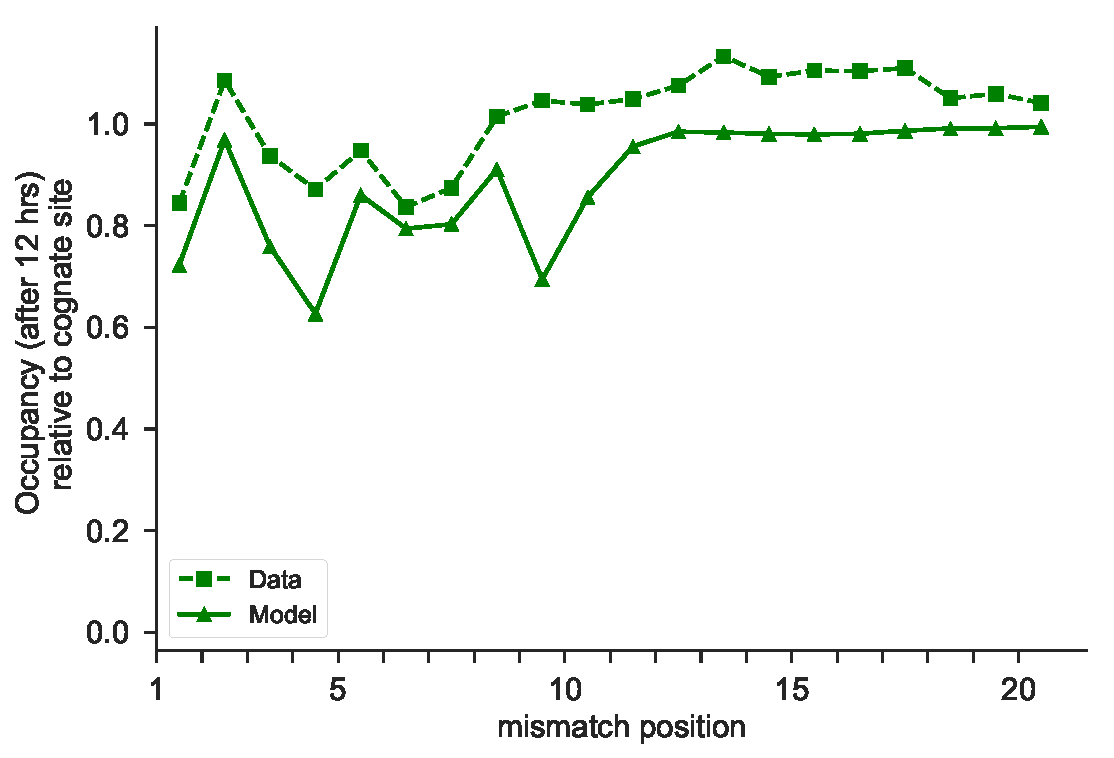
\includegraphics[scale=0.5]{fig25_10_10_2018.pdf}
\end{figure}

\begin{figure}[H]
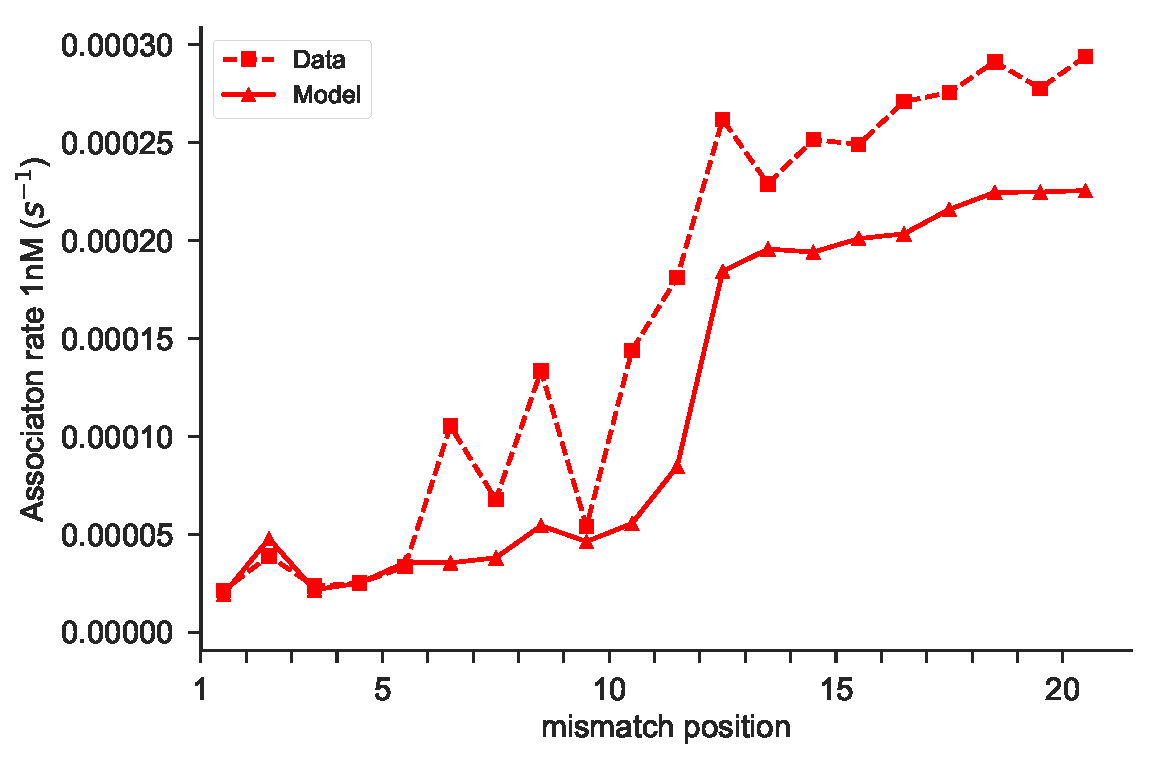
\includegraphics[scale=0.5]{fig26_10_10_2018.pdf}
\end{figure}

\begin{figure}[H]
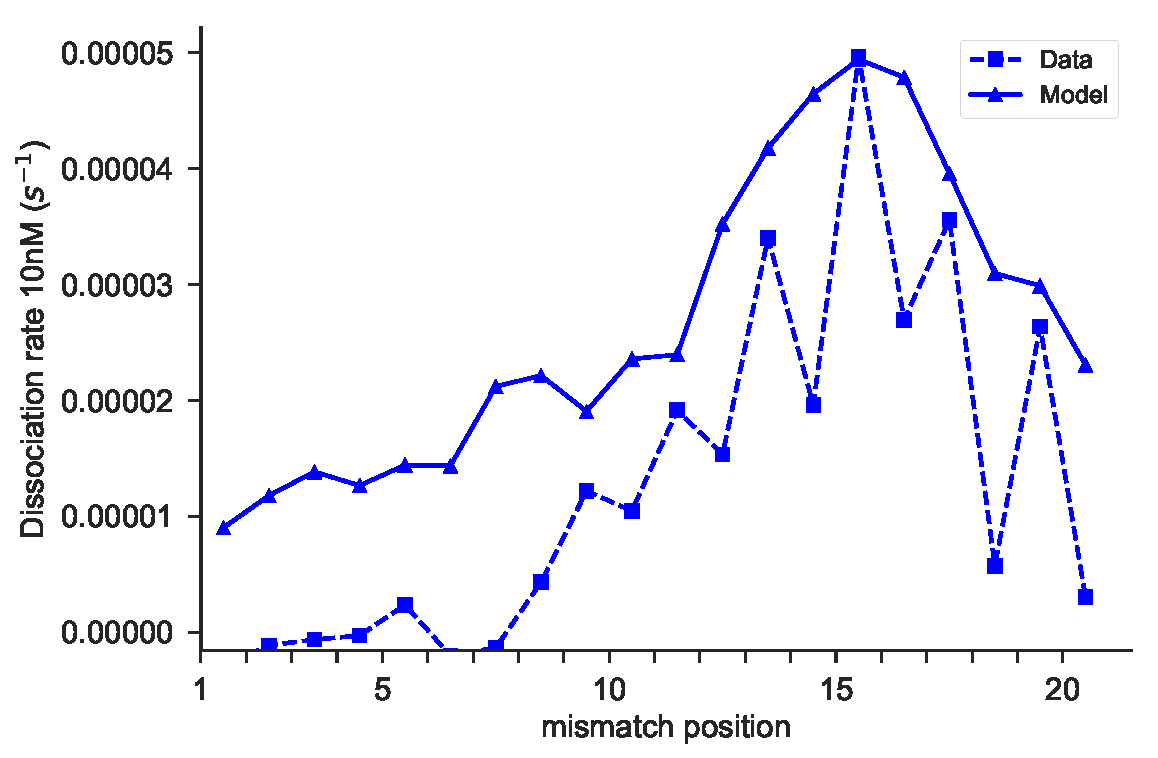
\includegraphics[scale=0.5]{fig27_10_10_2018.pdf}
\end{figure}

\begin{figure}[H]
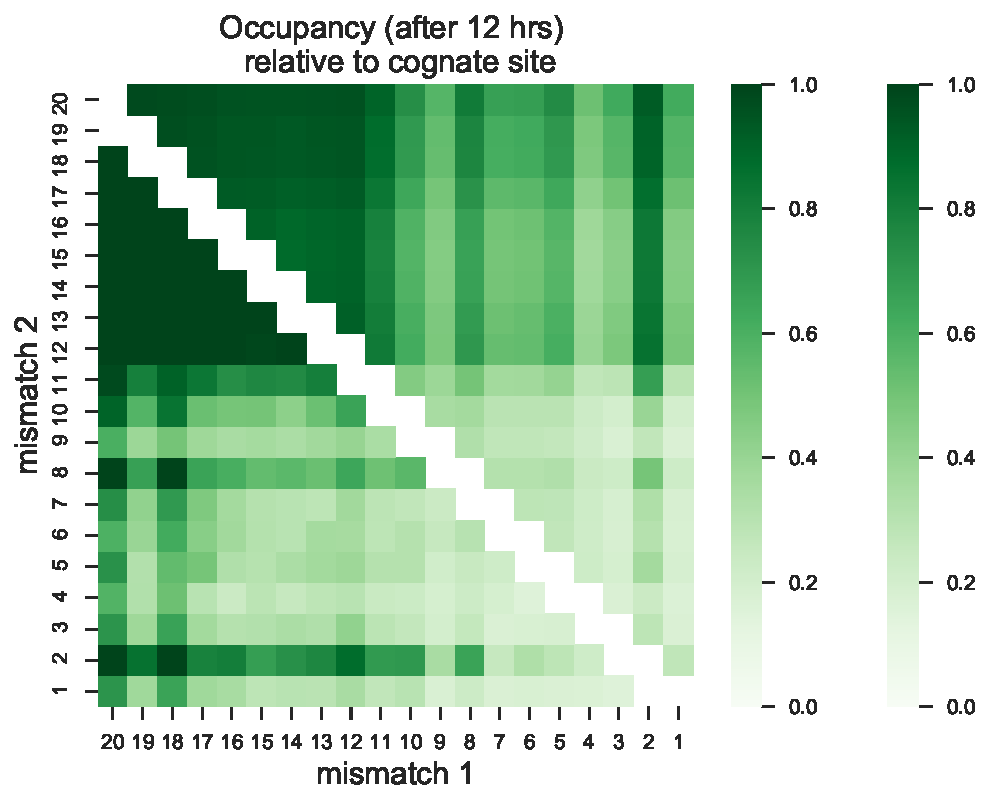
\includegraphics[scale=0.5]{fig28_10_10_2018.pdf}
\end{figure}

\begin{figure}[H]
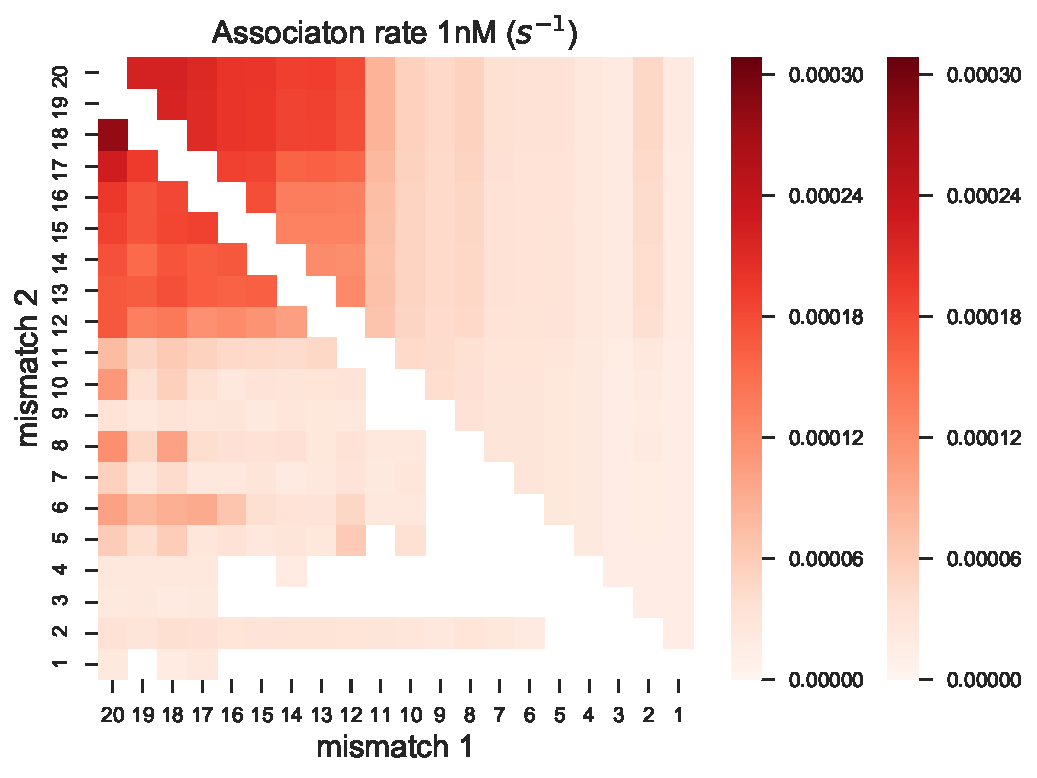
\includegraphics[scale=0.5]{fig29_10_10_2018.pdf}
\end{figure}

\begin{figure}[H]
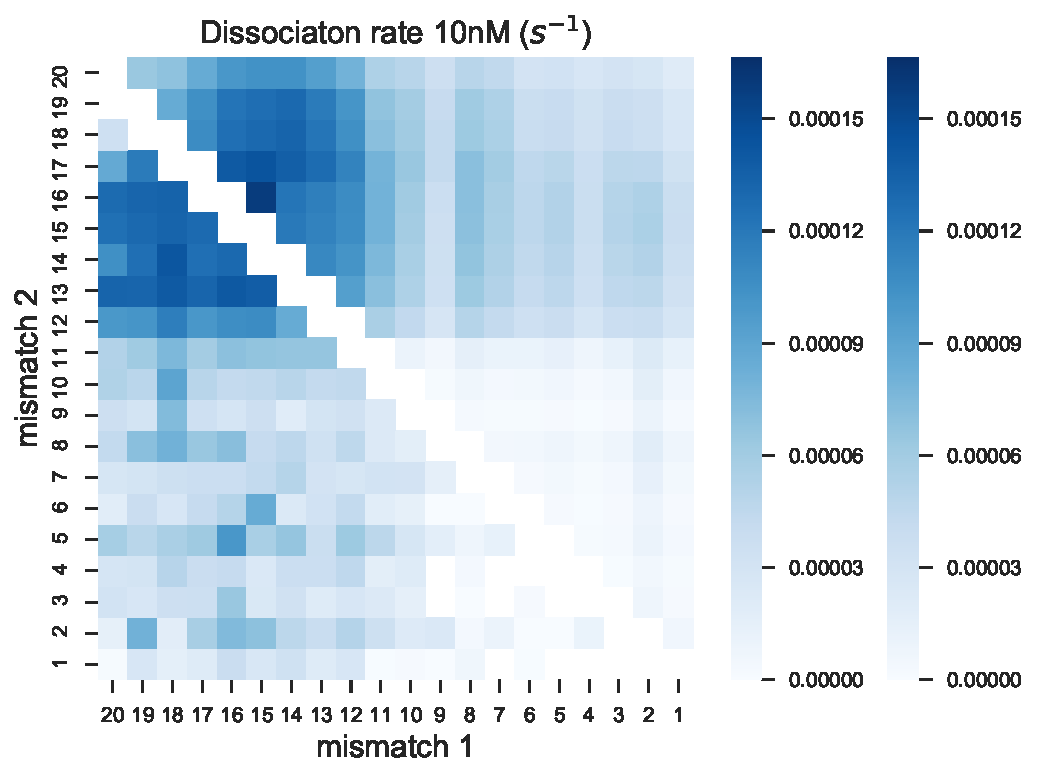
\includegraphics[scale=0.5]{fig30_10_10_2018.pdf}
\end{figure}


\subsection{class II: (near) constant $\epsilon_I$: No more statble states after second mismatch}

\begin{itemize}
\item If all datasets are included as training no fit directly resulted in something of this class. However, it consistently appears when we enforce a constant mismatch penalty (or when we ommit the dissociation data as will be made clear below). 
\item With these values, placing two (or more) mismatches destabilises the last state in the energy landscape. In other words: forming a full R-loop does not make the system more stable than the solution state.
\item  To fix the dissociation data, the on-target landscape exhibits a sharp dip around position 10. As we will show below, the dissociation data nessiciates that basically the entire gain in stability is placed in 1 step (see the graph of the bound free-energy/ (approx.) free-energy). 
\item The resulting free-energy landscape is not consistent with Ilya's data and does not even give such a good fit to Boyle's data.  
\item Still no good fit to the single-mismatch association data
\end{itemize}
\begin{figure}[H]
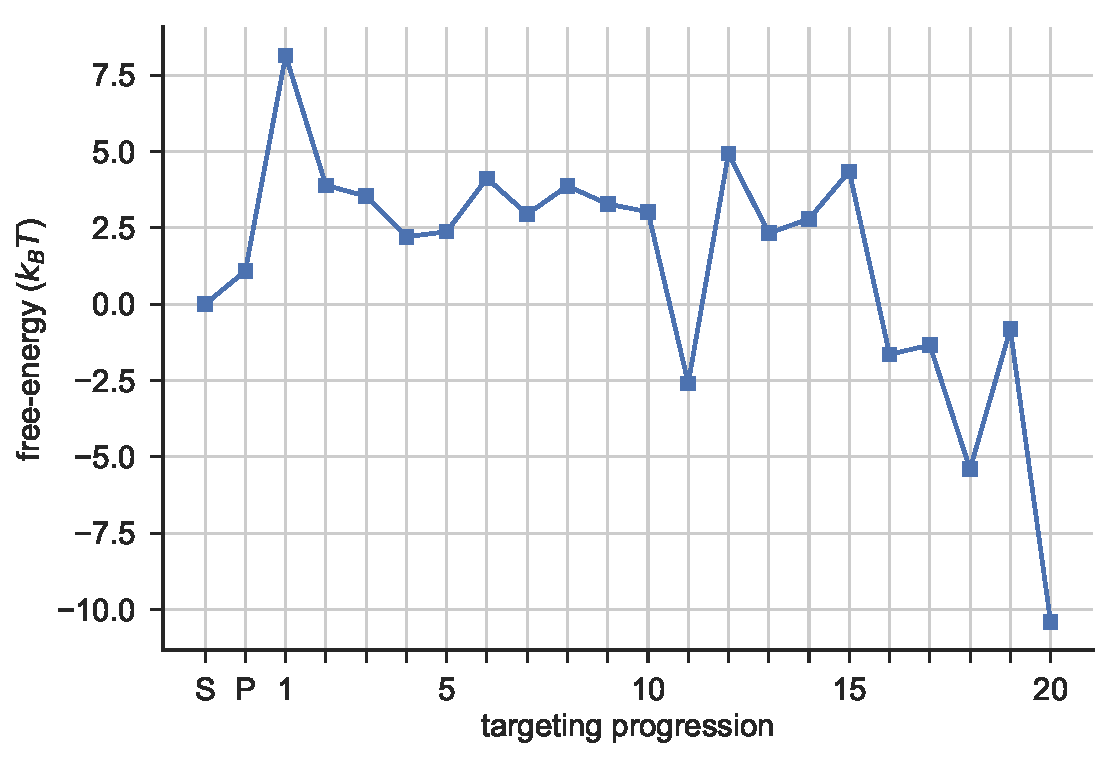
\includegraphics[scale=0.5]{fig32_10_10_2018.pdf}
\end{figure}


\begin{figure}[H]
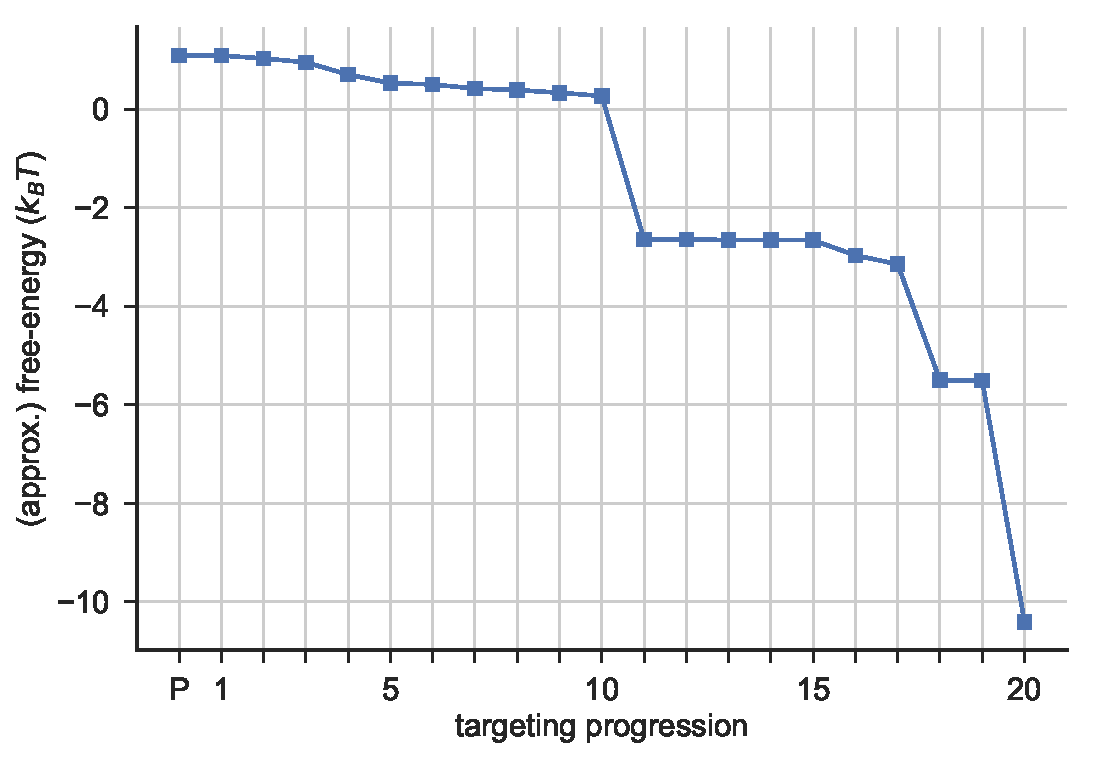
\includegraphics[scale=0.5]{fig40_10_10_2018.pdf}
\end{figure}

\begin{figure}[H]
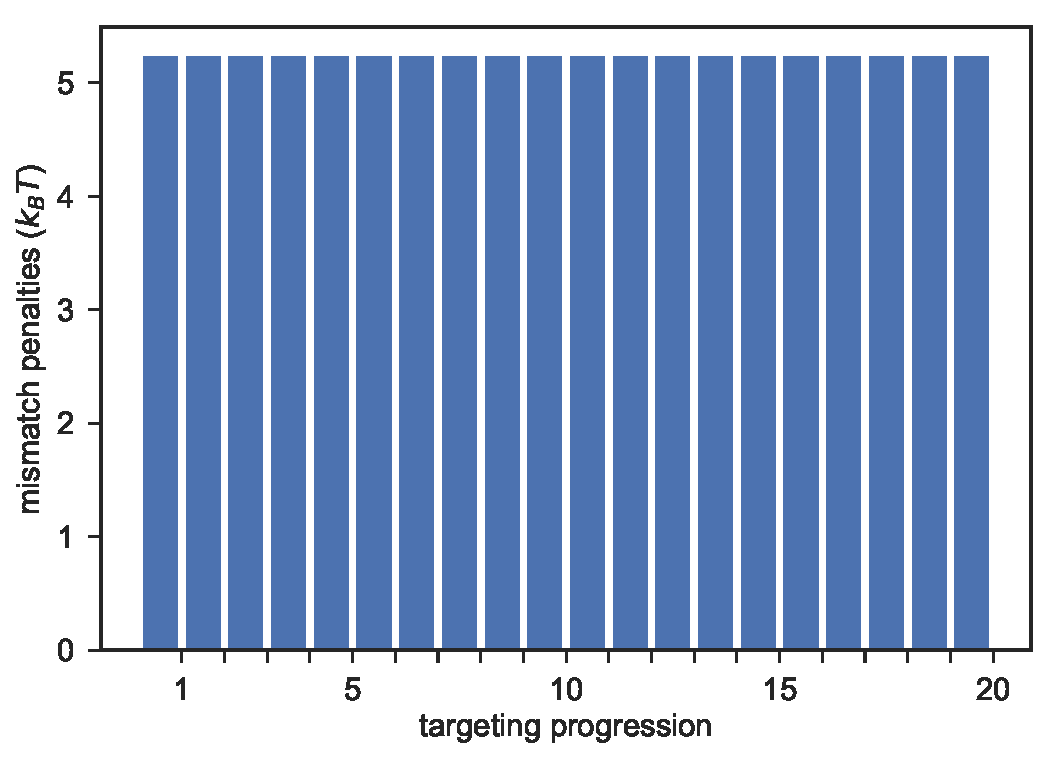
\includegraphics[scale=0.5]{fig33_10_10_2018.pdf}
\end{figure}

\begin{figure}[H]
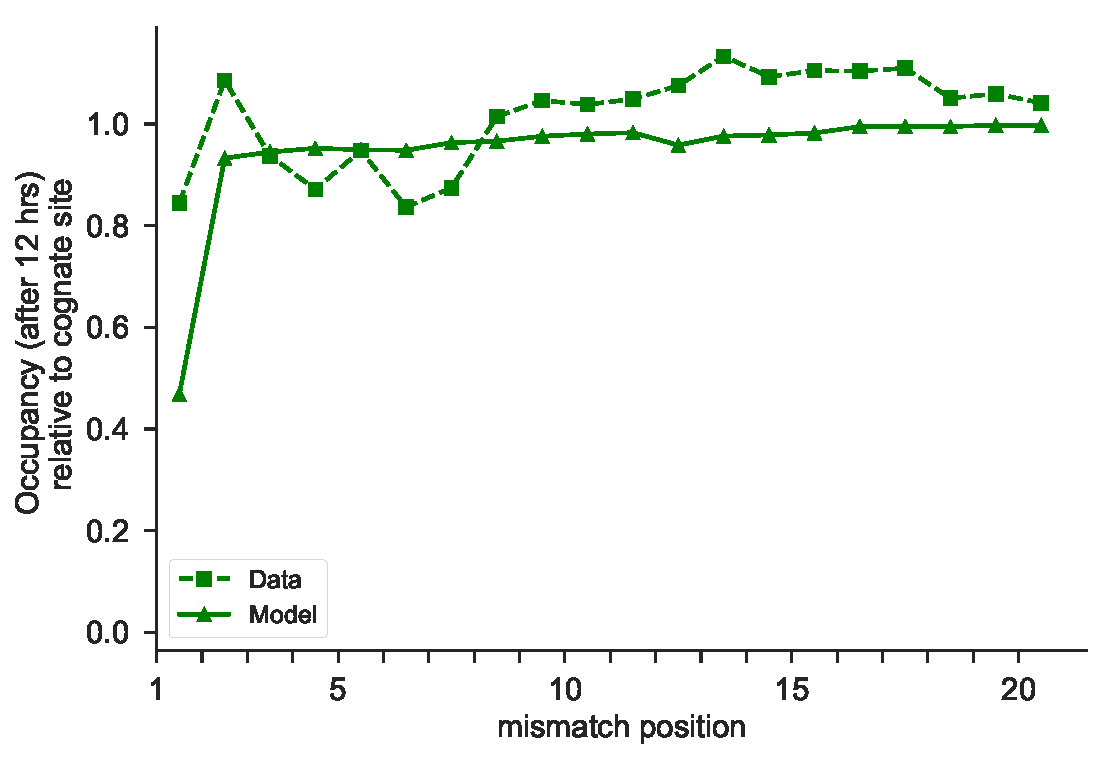
\includegraphics[scale=0.5]{fig34_10_10_2018.pdf}
\end{figure}

\begin{figure}[H]
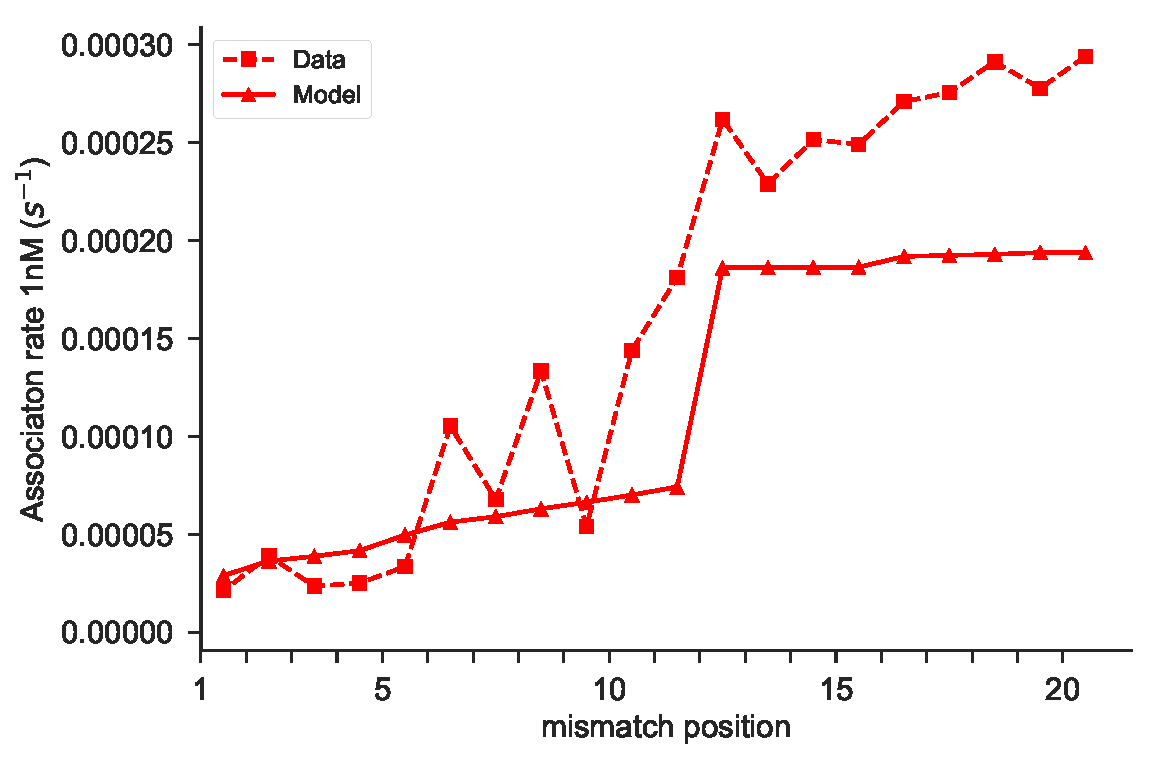
\includegraphics[scale=0.5]{fig35_10_10_2018.pdf}
\end{figure}

\begin{figure}[H]
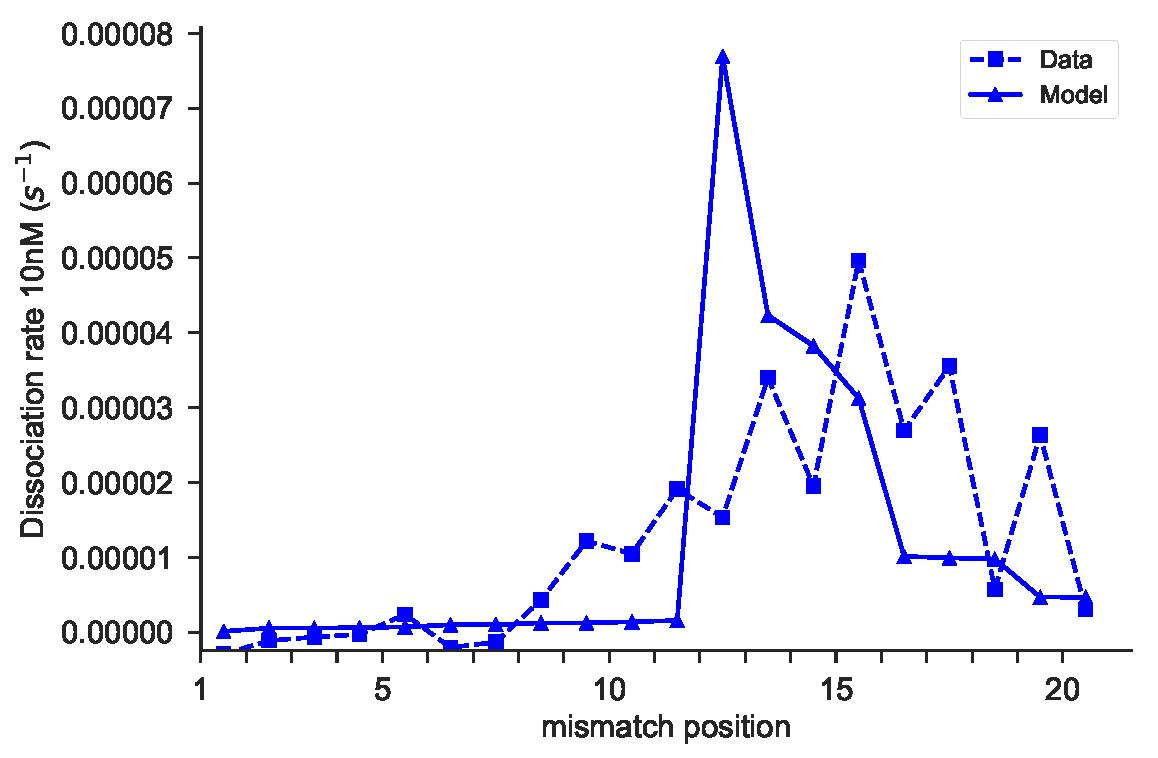
\includegraphics[scale=0.5]{fig36_10_10_2018.pdf}
\end{figure}

\begin{figure}[H]
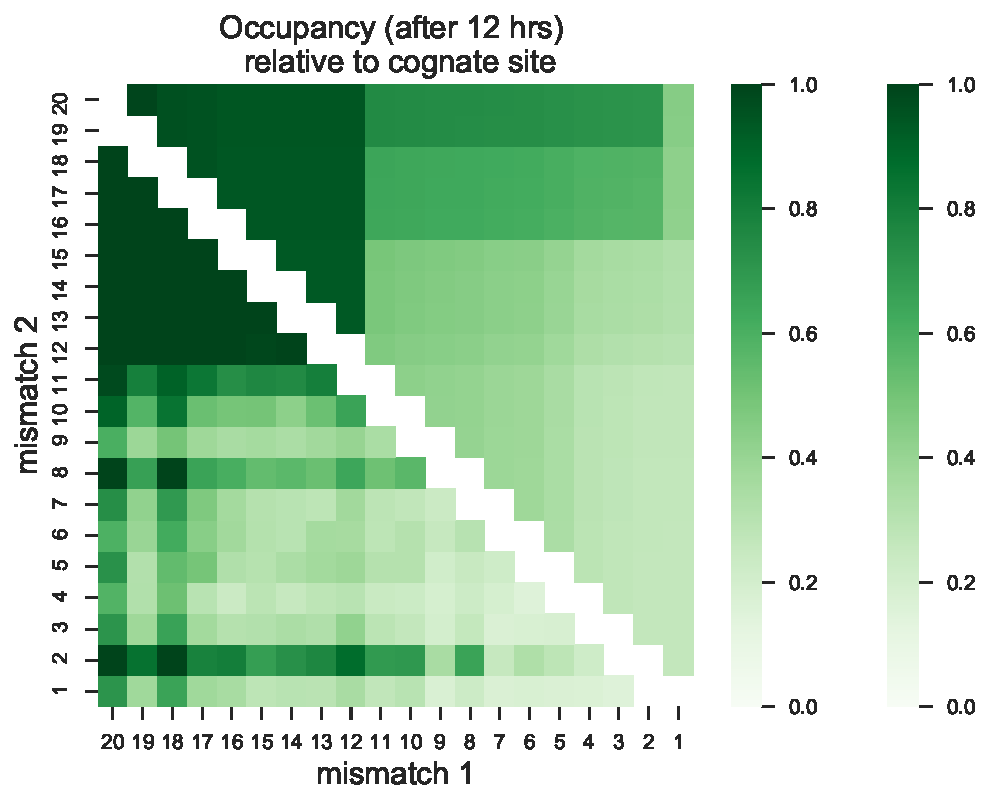
\includegraphics[scale=0.5]{fig37_10_10_2018.pdf}
\end{figure}

\begin{figure}[H]
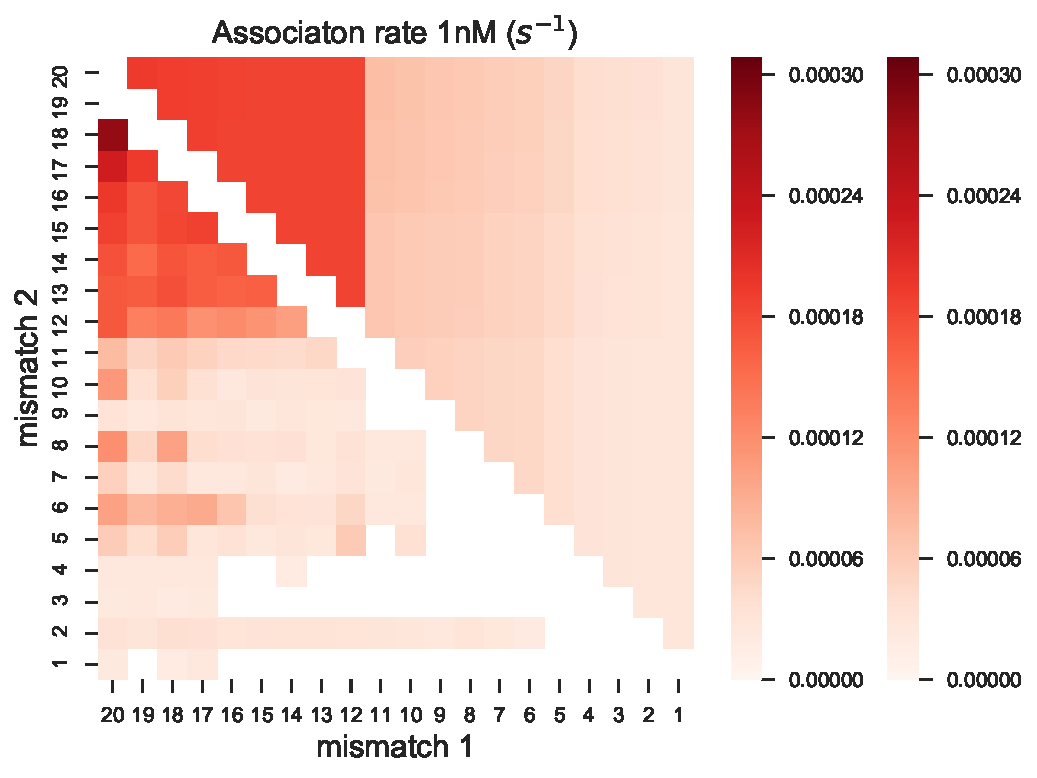
\includegraphics[scale=0.5]{fig38_10_10_2018.pdf}
\end{figure}

\begin{figure}[H]
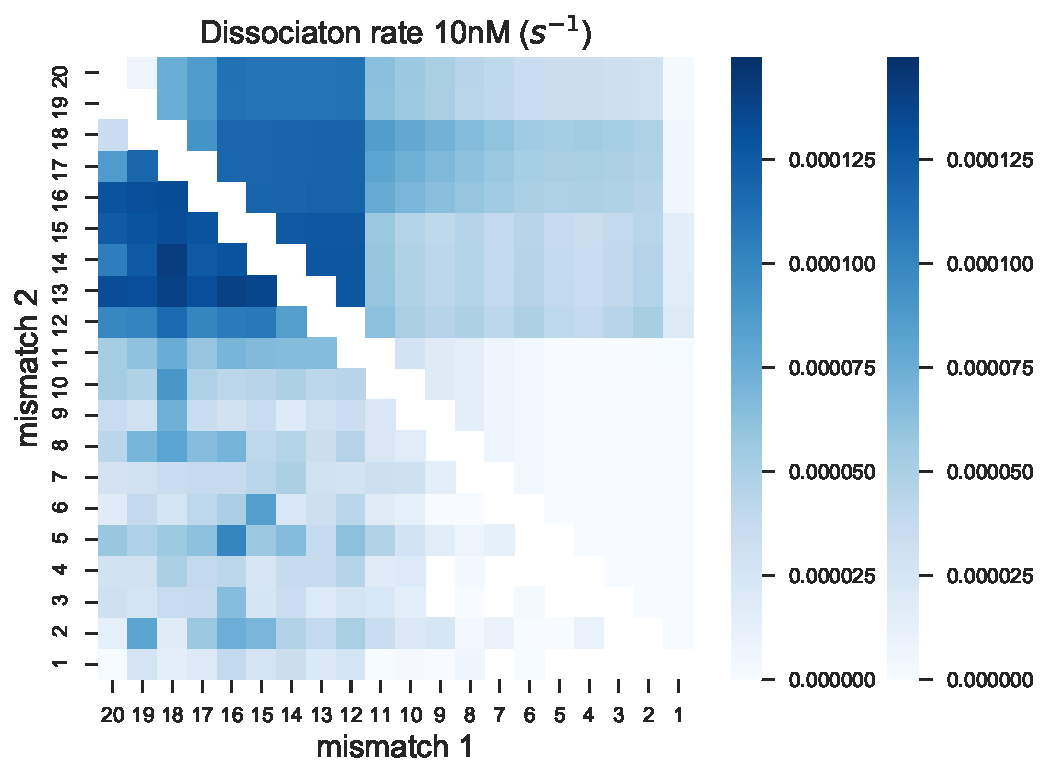
\includegraphics[scale=0.5]{fig39_10_10_2018.pdf}
\end{figure}
\section{Hints from data: "two-state" approximation}
\begin{itemize}
\item Clearly, placing more than two mismatches does not alter the rates and occupancy further (see figures further down in this section). 
\item Also, the data is similar to that of the mismatches placed after each other.
\item Explanation: an effective two-state system when more than one mismatch is placed.
\item We imagine all mismatches to be placed straight after each other.
\item Also, the system has no stable states from the (second) mismatch onwards. In other words, from two mismatches on, we can imagine there to be mismatches all the way through the hybrid from the first mismatches' position. 
\item The R-loop will form until the mismatches (before the block)
\item Two-states: Solution (or PAM) and the matching part of the R-loop
\end{itemize}

\begin{figure}[H]
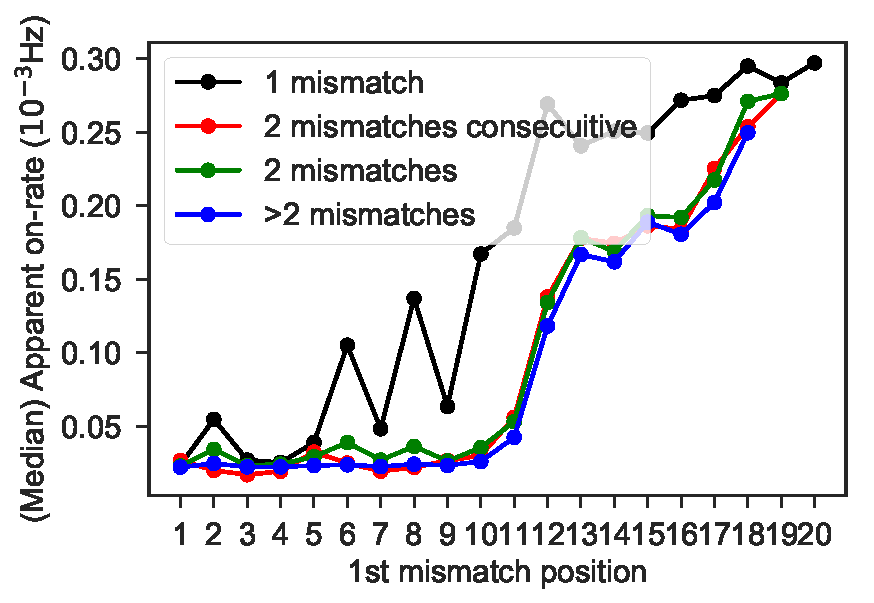
\includegraphics[scale=0.5]{fig1_10_10_2018.pdf}
\end{figure}

\begin{figure}[H]
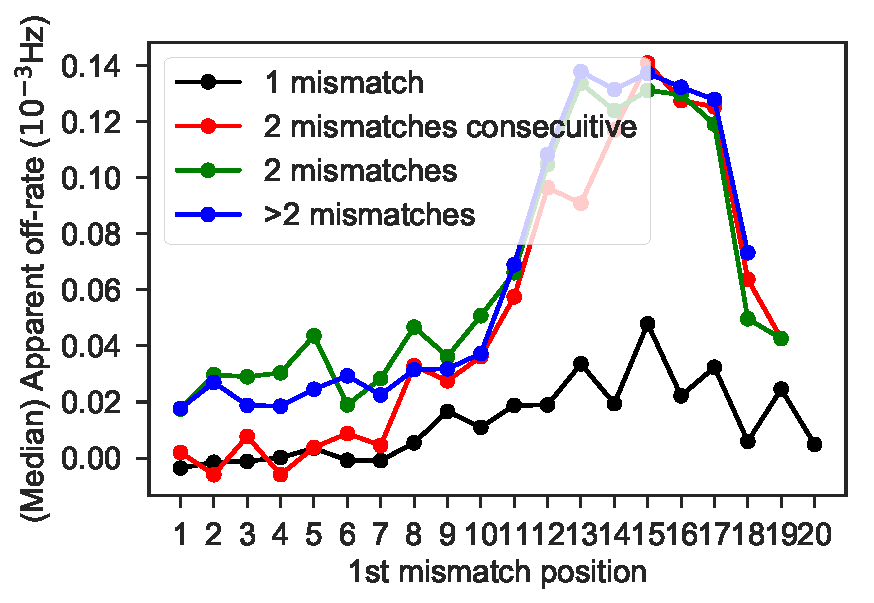
\includegraphics[scale=0.5]{fig2_10_10_2018.pdf}
\end{figure}

\begin{figure}[H]
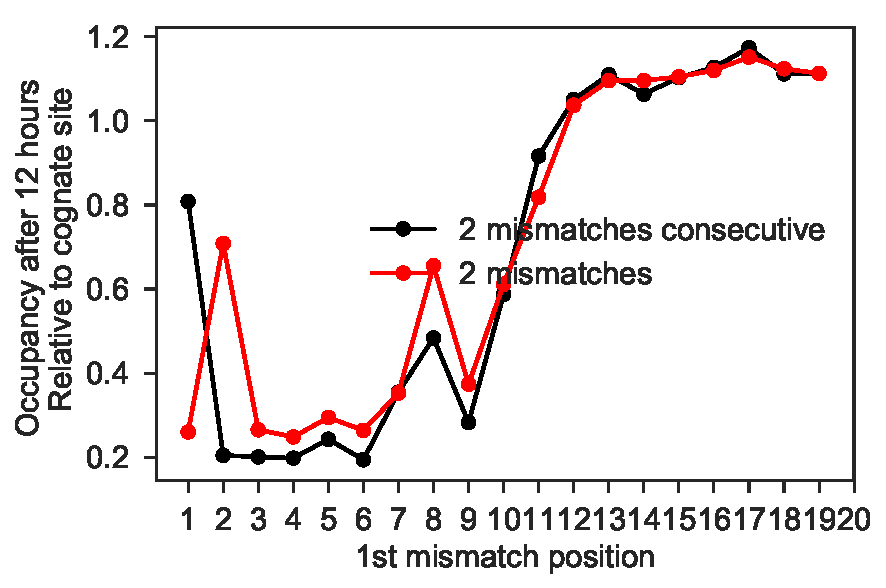
\includegraphics[scale=0.5]{fig3_10_10_2018.pdf}
\end{figure}

\section{Toy Model: Two-state system}


\begin{itemize}
\item Clearly, the data says we need the parameter regime of 'class II'. 
\item However, we keep failing at getting a consistent fit to all available data.
\item We therefore constructed a little two-state 'Toy-Model' to see - given class II - which datasets are actually numerically comptable with one another. 
\item Solving Master Equation for two-state system:
\begin{equation}
P_{on}(t) = \frac{\rate{on}}{ \rate{on} + \rate{off}} \left(1 - e^{-(\rate{on}+\rate{off})t} \right)
\end{equation}
\end{itemize}


\subsection{Predict based on association data}

\begin{itemize}
\item Assume that the on-rate cannot be sequence dependent. Therefore $\rate{on}$ can be estimated based on the measured association rate for the cognate target.
\item The association rate is measured by fitting a line through the points $P(t=500)$, $P(t=1000)$ and $P(t=1500)$ and enforcing it to go through the origin. If $P(t)$ is based on the above equation, the association rate equals $\rate{two-state}$, a function of $\rate{on}$ - which is known -  and $\rate{off}$.
\item For every measured association rate. Invert - numerically solve for the roots of - 
\begin{equation}
\rate{asso} - \rate{two-state} = 0 
\end{equation} 
\item this gives an estimated off-rate, $\rate{off}$, for every association rate 
\item use the $\rate{off}$ values to estimate the dissociation rate (as measured):
\begin{equation}
P_{on}(t) \approx e^{-\rate{off}t}
\end{equation}
assuming the two-state approximation. The dissociation rate is again the product of a linear fit to three time points. 
\item use the $\rate{off}$ values to estimate the free-energy landscape of the on-target. Given the block of mismatches destabilizes the system after it, the free-energy landscape can be constructed by combining the truncated systems. In other words: first mismatch pos 2-20, then 3-20, 4-20, etc. 
\begin{equation}
\Delta F_n \approx \log(\rate{off}(n))
\end{equation}
with $\rate{off}(n)$ the off-rate from a target with mismatches from position $n$ onwards.
\item use the $\rate{off}$ values to predict the occupancy after $T=$12hrs:
\begin{equation}
P_{on}(12hrs) = \frac{\rate{on}}{ \rate{on} + \rate{off}} \left(1 - e^{-(\rate{on}+\rate{off})12*3600} \right)
\end{equation} 
\end{itemize}


\begin{figure}[H]
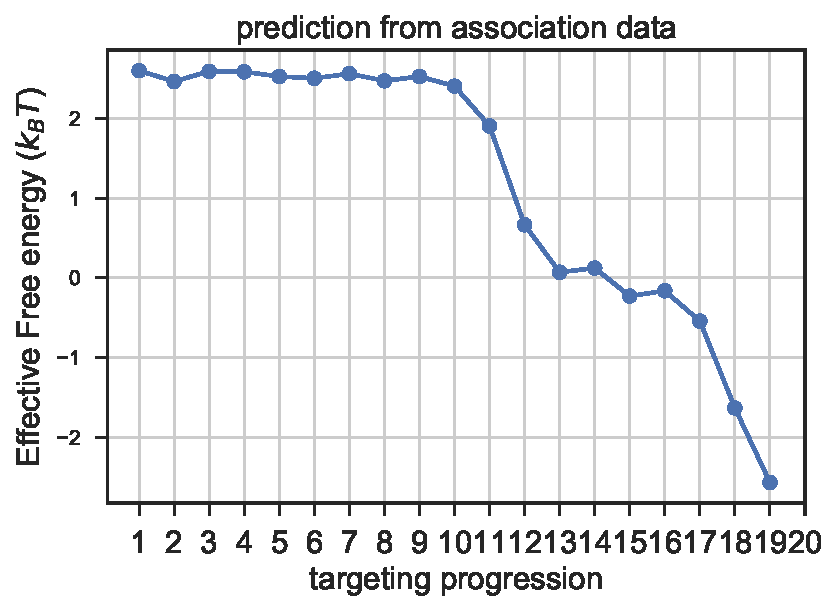
\includegraphics[scale=0.5]{fig5_10_10_2018.pdf}
\end{figure}

\begin{figure}[H]
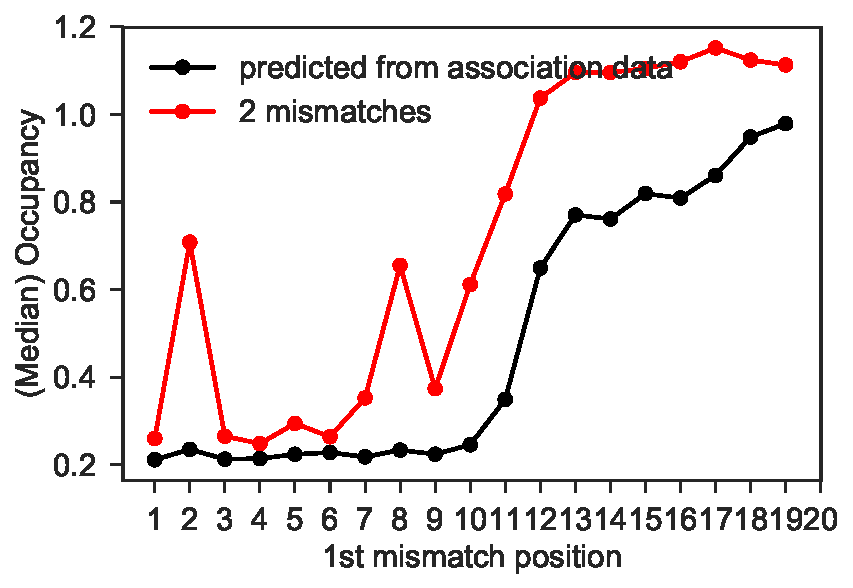
\includegraphics[scale=0.5]{fig6_10_10_2018.pdf}
\end{figure}

\begin{figure}[H]
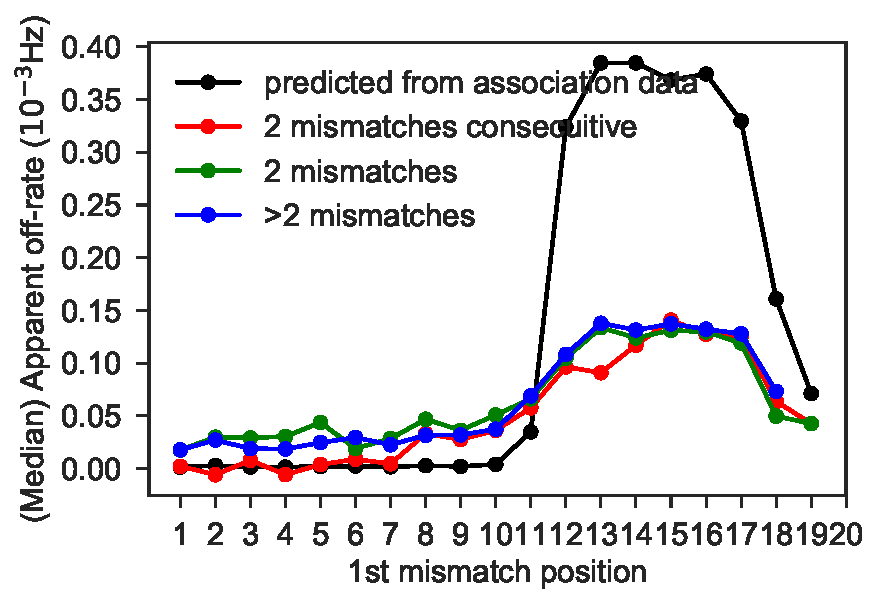
\includegraphics[scale=0.5]{fig7_10_10_2018.pdf}
\end{figure}


Conclusion: Although no quantitative agreement is achieved, qualitatively the association rate is a decent predictor of the other data. 

\subsection{Predict based on dissociation data}
\begin{itemize}
\item This time we have the measured dissocation rates from which we can - again by root solving - obtain the $\rate{off}$ values 
\item from here we can convert it to assocation rates and occupancies. 
\item Only thing is, there is a catch: There are two roots ($\rate{off}$ values) for every dissocation rate:
\end{itemize}


\begin{figure}[H]
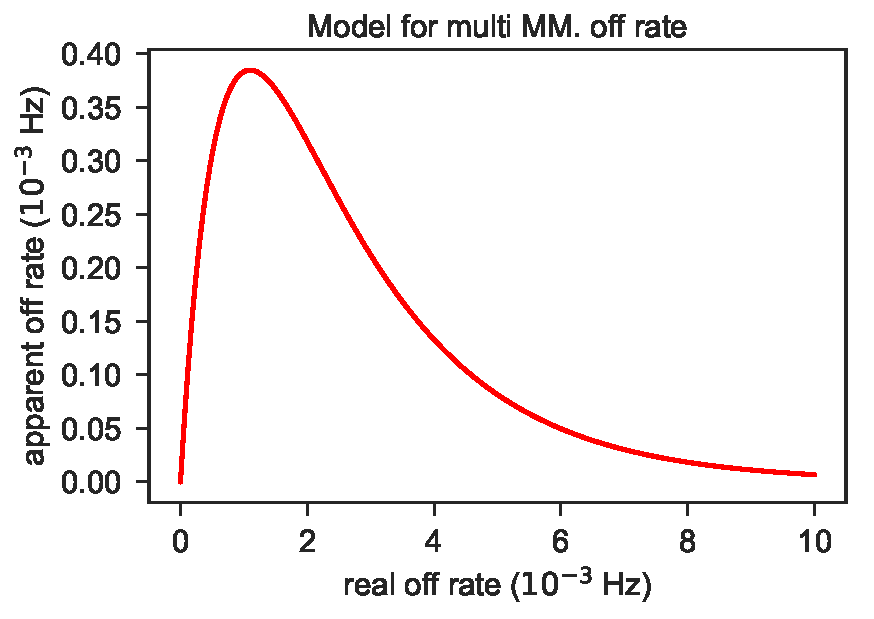
\includegraphics[scale=0.5]{fig8_10_10_2018.pdf}
\end{figure}

\begin{figure}[H]
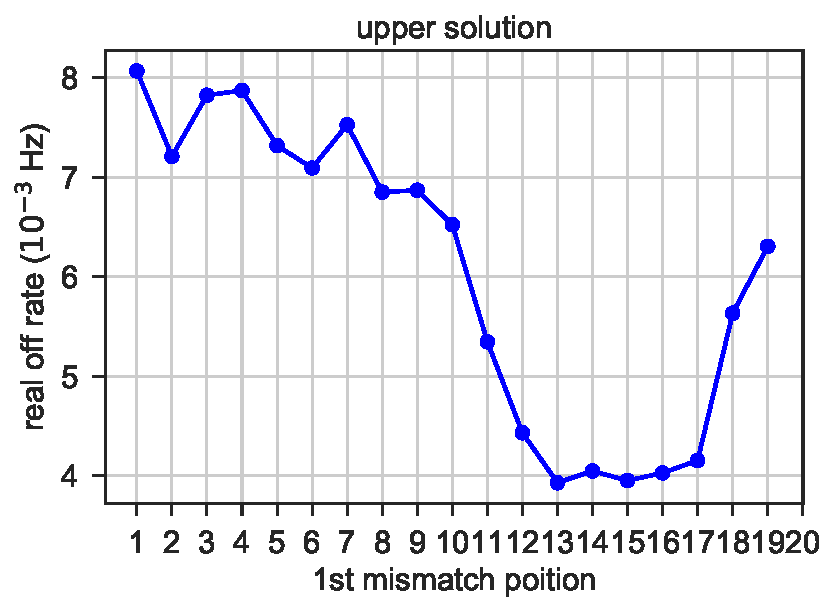
\includegraphics[scale=0.5]{fig9_10_10_2018.pdf}
\end{figure}
\begin{figure}[H]
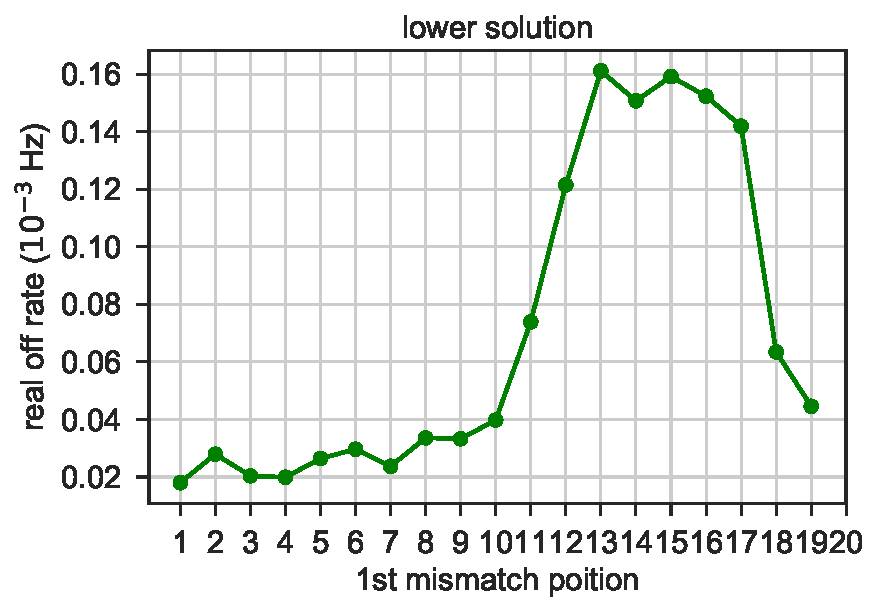
\includegraphics[scale=0.5]{fig10_10_10_2018.pdf}
\end{figure}

\begin{itemize}
\item Hence, after finding both roots we must have a way of deciding which root to use when constructing the free-energy landscape. 
\item The free-energy is a monotonically decreasing function. Therefore, so must the $\rate{off}$ - enforcing us to (at least once) switch between the two possible roots. 
\item Starting from the upper solution, we see that there are essentially two choices we can make. Either switch around 18 or around 13. 
\item no mater what choice - switch at 18 not shown - the largest drop in free energy will be whenever this switch is made. 
\item Long story short... The dissociation data can only be reproduced (quantitatively) if there is 1 single large drop in (free-)energy.
\item As the free-energy after this drop remains rather constant, the $\epsilon_C$ values should actually be high again: This gives that "zig-zag-like" pattern in the Simulated Annealing fits.  
\end{itemize}

\begin{figure}[H]
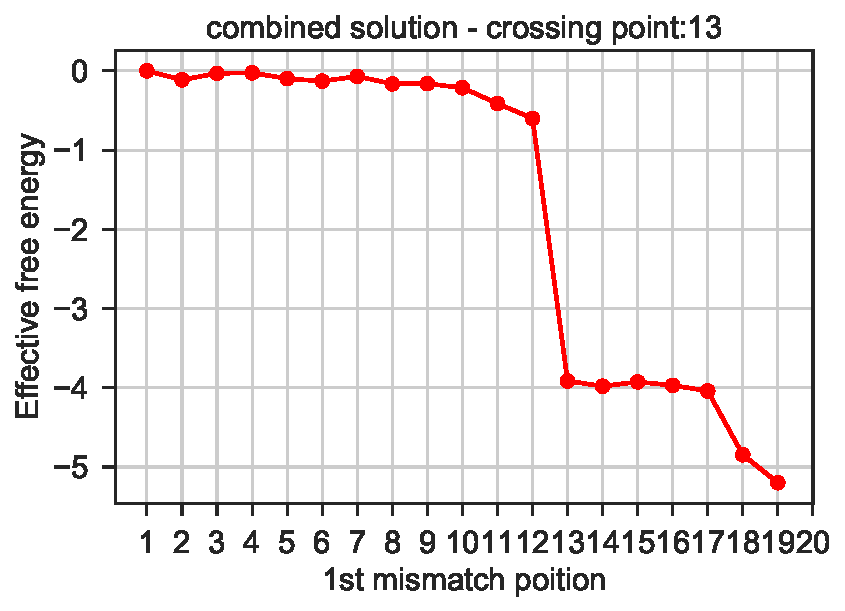
\includegraphics[scale=0.5]{fig11_10_10_2018.pdf}
\end{figure}

Conclusion: Clearly, the dissociation rate cannot be used as a predictor of the association data and occupancy data.  The numbers are simply incompatible. 

\subsection{Predict based on occupancy data}
\begin{itemize}
\item using the occupation data we obtain the free-energy using (assuming equilibration): 
\begin{equation}
P(\Delta F) = \frac{1}{1 + e^{-\Delta F}}
\end{equation}
with the solution having an energy of zero. 
\item From here on, we can convert it to assocation and dissociation rates. First we obtain the $\rate{off}$ values. 

\begin{equation}
\frac{\rate{on}^{OT}}{\rate{off}} = \frac{P_{off}}{P_{on}} = e^{-\Delta F}
\end{equation}

\item Then, we can estimate the association rate from the $\rate{off}$ values - by once again performing the proper linear fit. 
\end{itemize}


\begin{figure}[H]
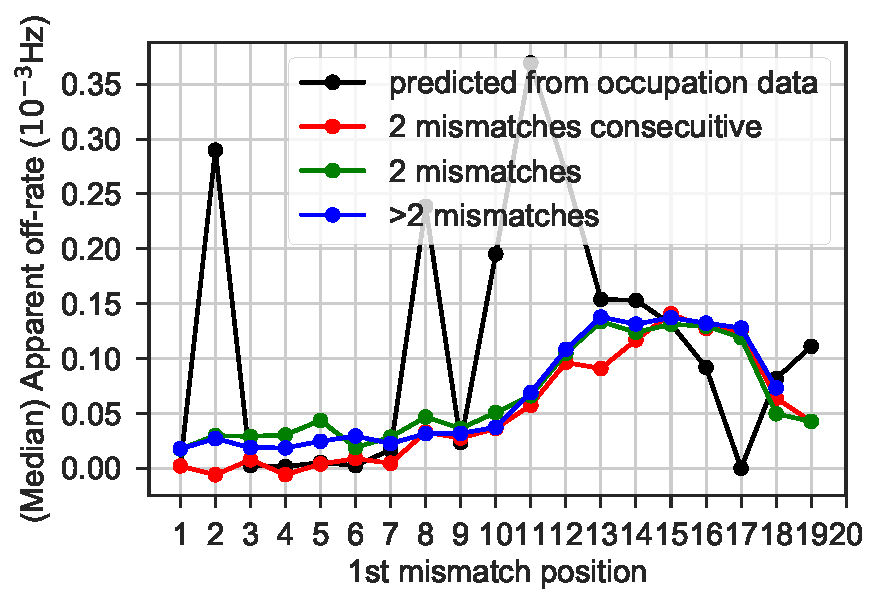
\includegraphics[scale=0.5]{fig12_10_10_2018.pdf}
\end{figure}
\begin{figure}[H]
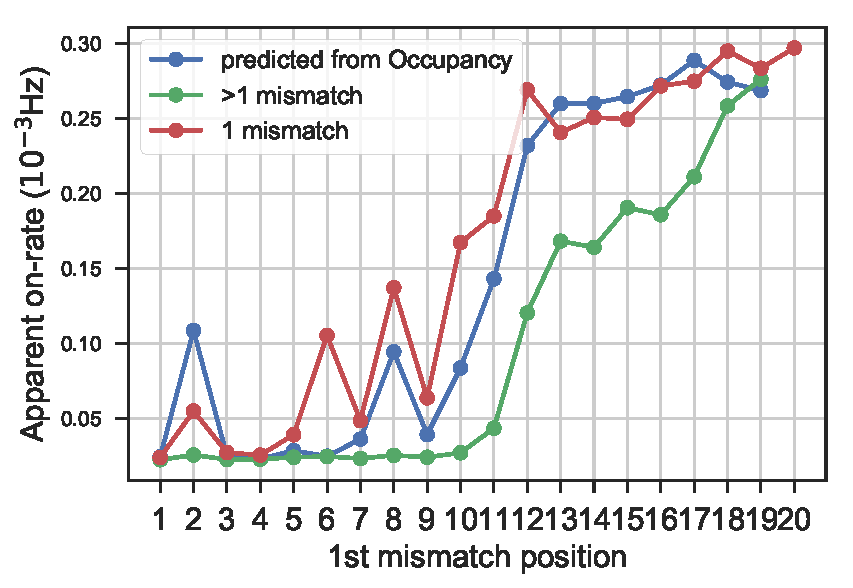
\includegraphics[scale=0.5]{fig13_10_10_2018.pdf}
\end{figure}


Conclusion: The occupancy data does not contain temporal information. Hence, these numbers cannot be used to accurately predict the association and dissociation data.
\section{Simmulated Annealing: Fit to association data confirms two-state approximation holds}
\begin{itemize}
\item Fit only to association data (above analysis indicated that this should at least give correct shape of landscape).
\item We even get a consistent fit to both single and double (hence multiple) mismatch association rate data.
\item Results from the fit look, qualitatively, similar to those from the Toy-model analysis shown above.
\item Note that only the association rate is fitted. All other plots actually are predictions.
\item FYI: We had quite loose bounds for the rates and the fit decided to use such large numbers that sometimes the occupancy spikes above 1 due to numerical errors in the algorithm for the matrix exponential. We started a fit with tighter bounds.. no worries :). 
\end{itemize}


\begin{figure}[H]
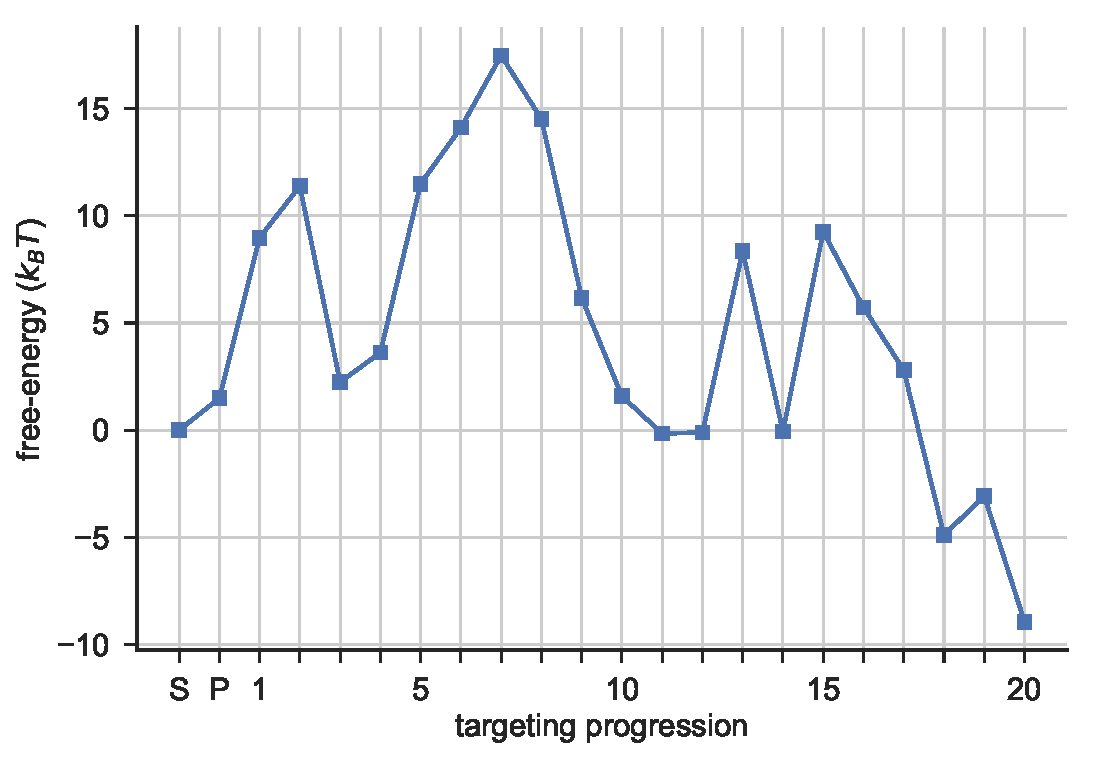
\includegraphics[scale=0.5]{fig14_10_10_2018.pdf}
\end{figure}


\begin{figure}[H]
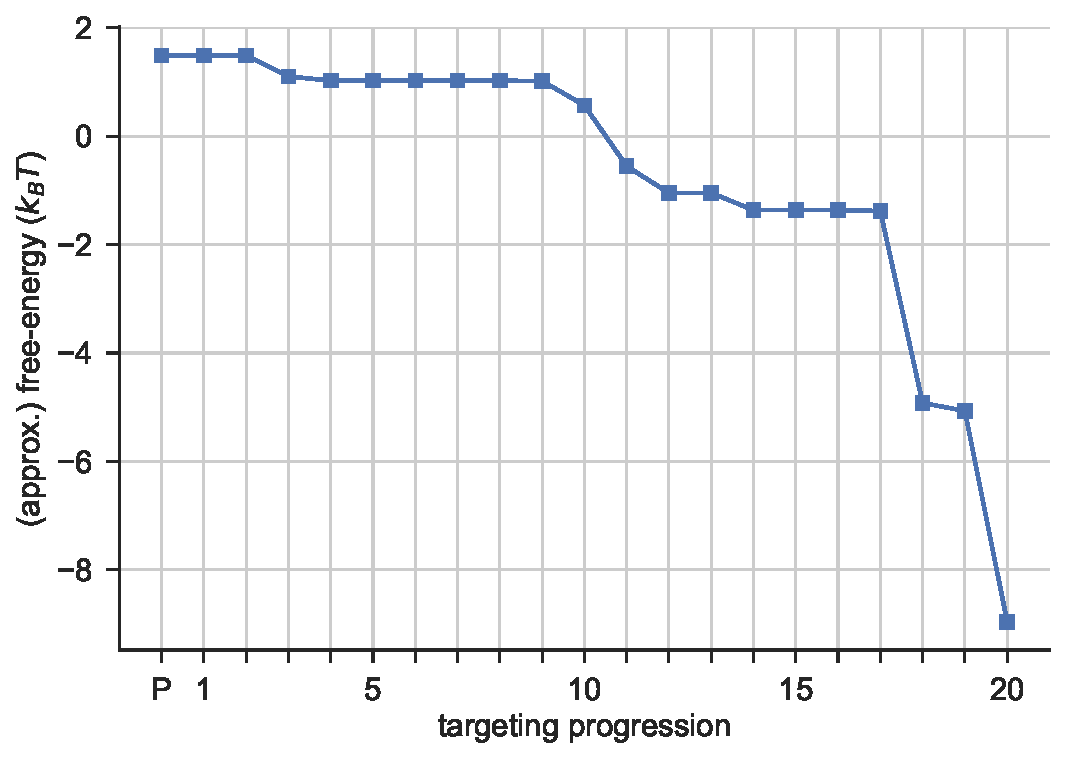
\includegraphics[scale=0.5]{fig15_10_10_2018.pdf}
\end{figure}


\begin{figure}[H]
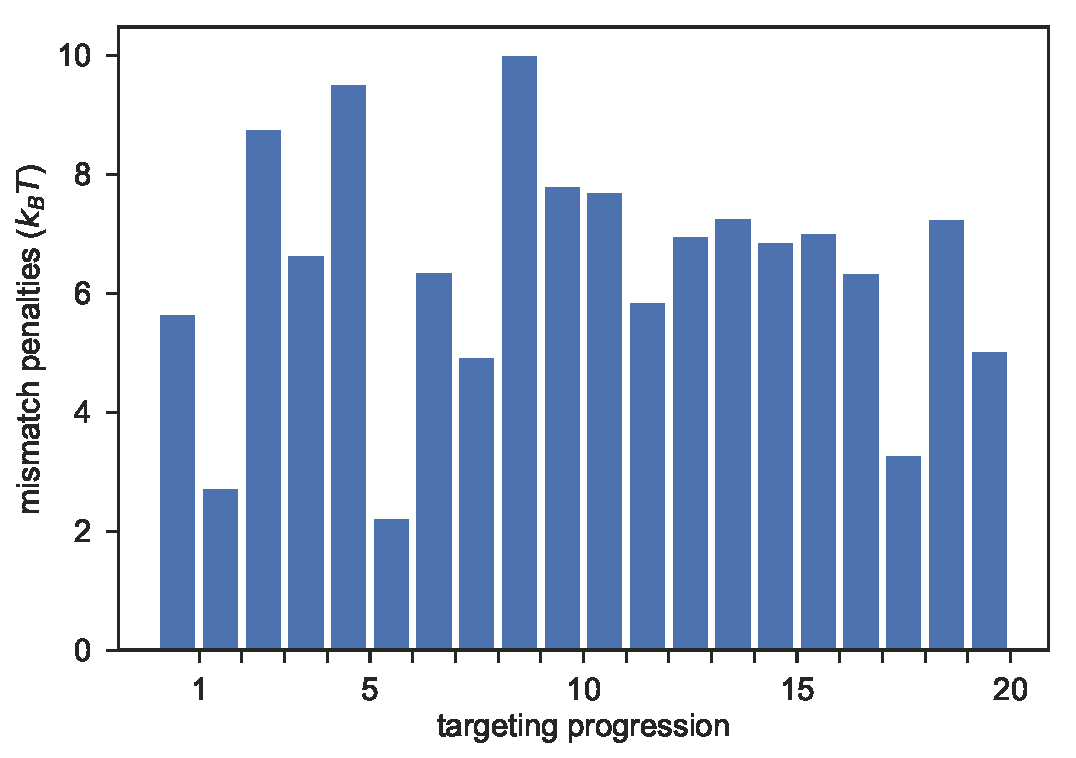
\includegraphics[scale=0.5]{fig16_10_10_2018.pdf}
\end{figure}

\begin{figure}[H]
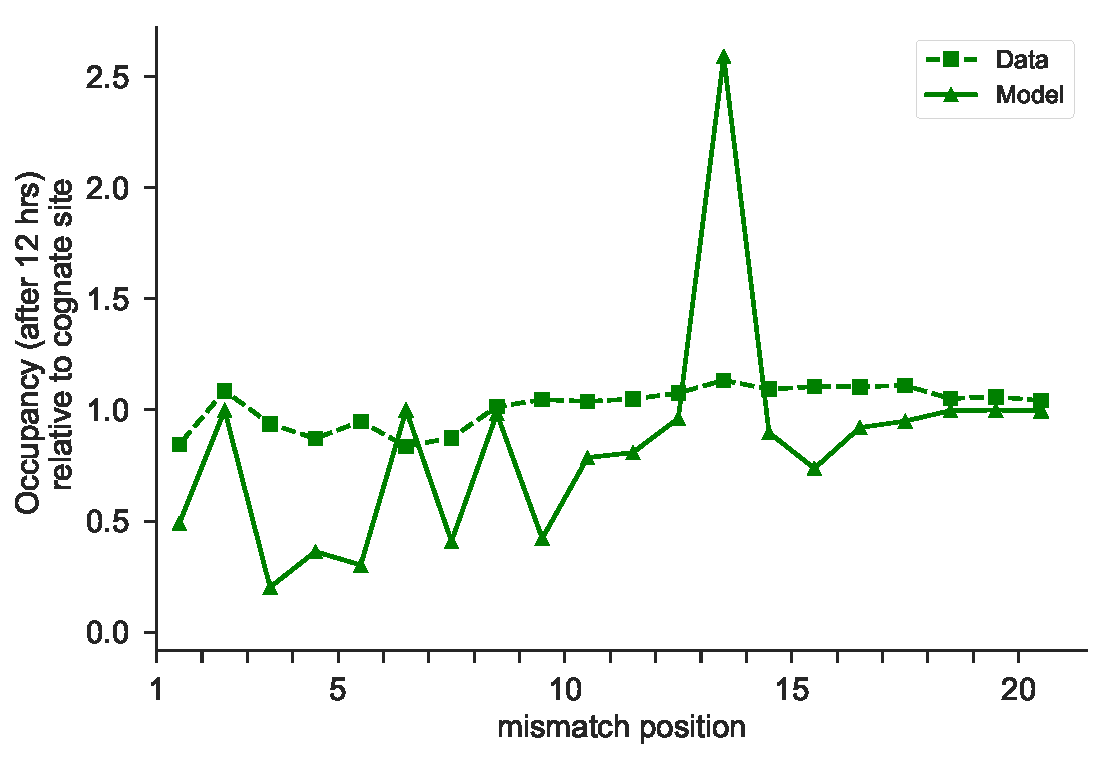
\includegraphics[scale=0.5]{fig17_10_10_2018.pdf}
\end{figure}

\begin{figure}[H]
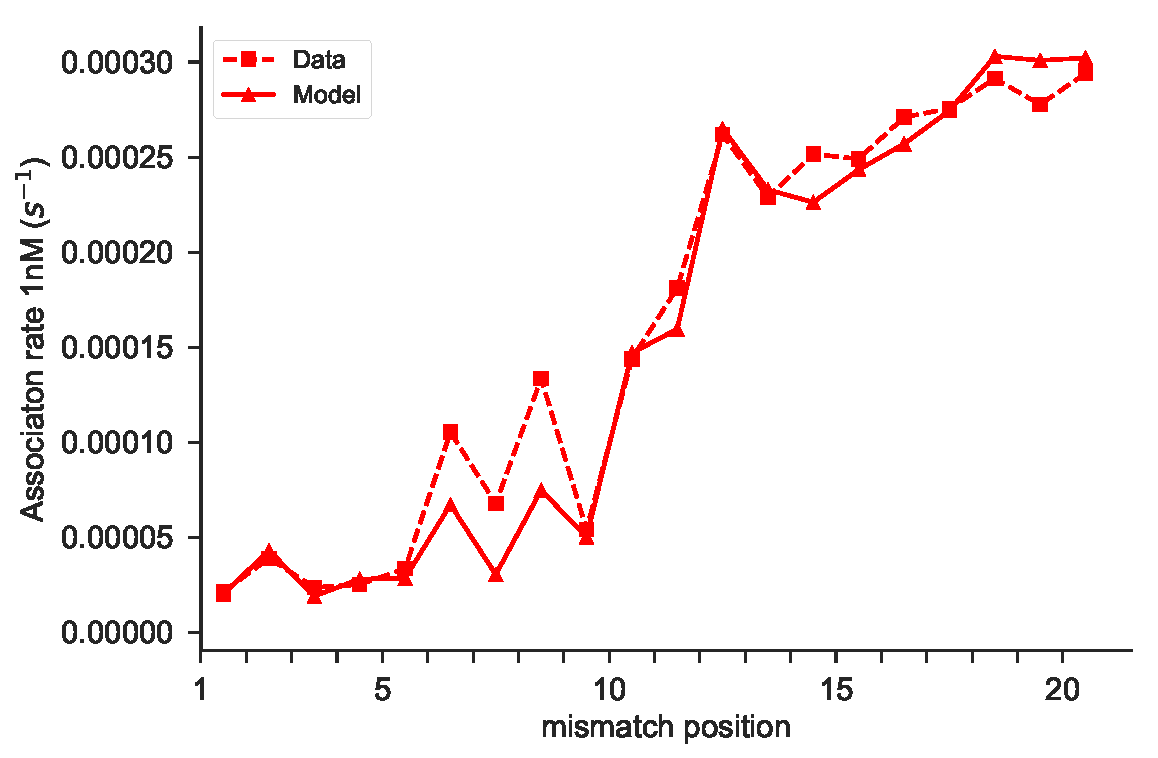
\includegraphics[scale=0.5]{fig18_10_10_2018.pdf}
\end{figure}


\begin{figure}[H]
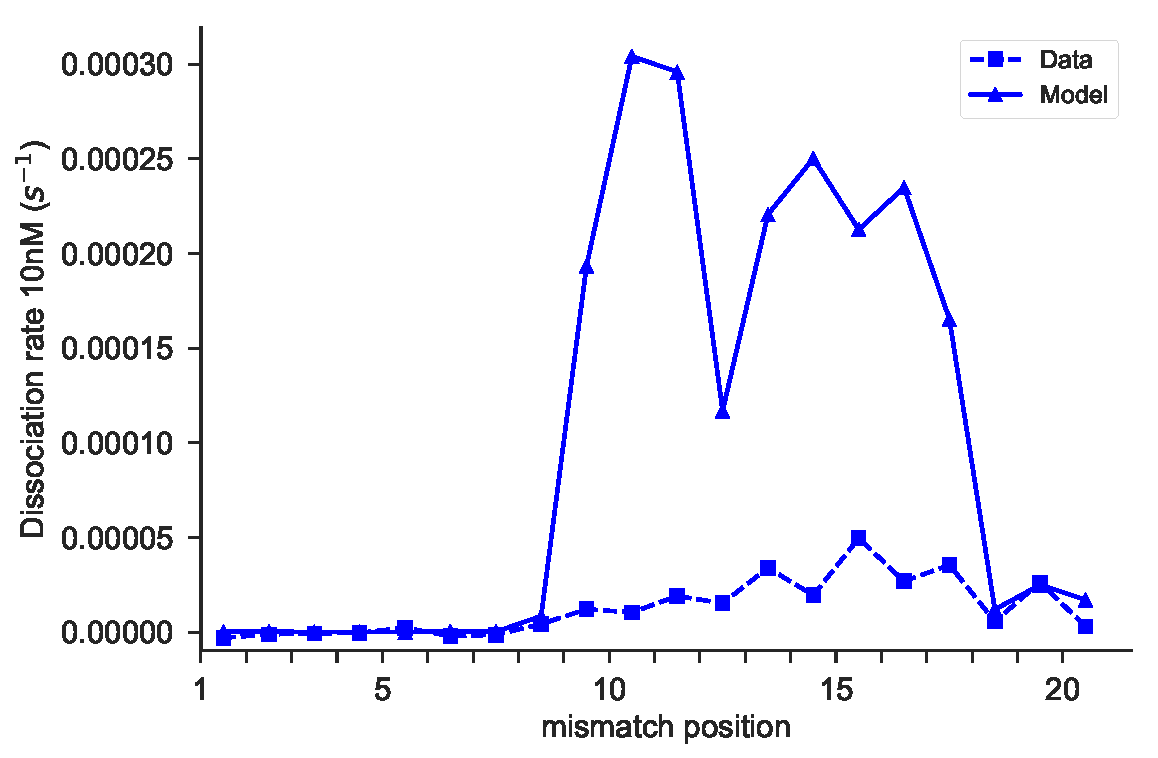
\includegraphics[scale=0.5]{fig19_10_10_2018.pdf}
\end{figure}


\begin{figure}[H]
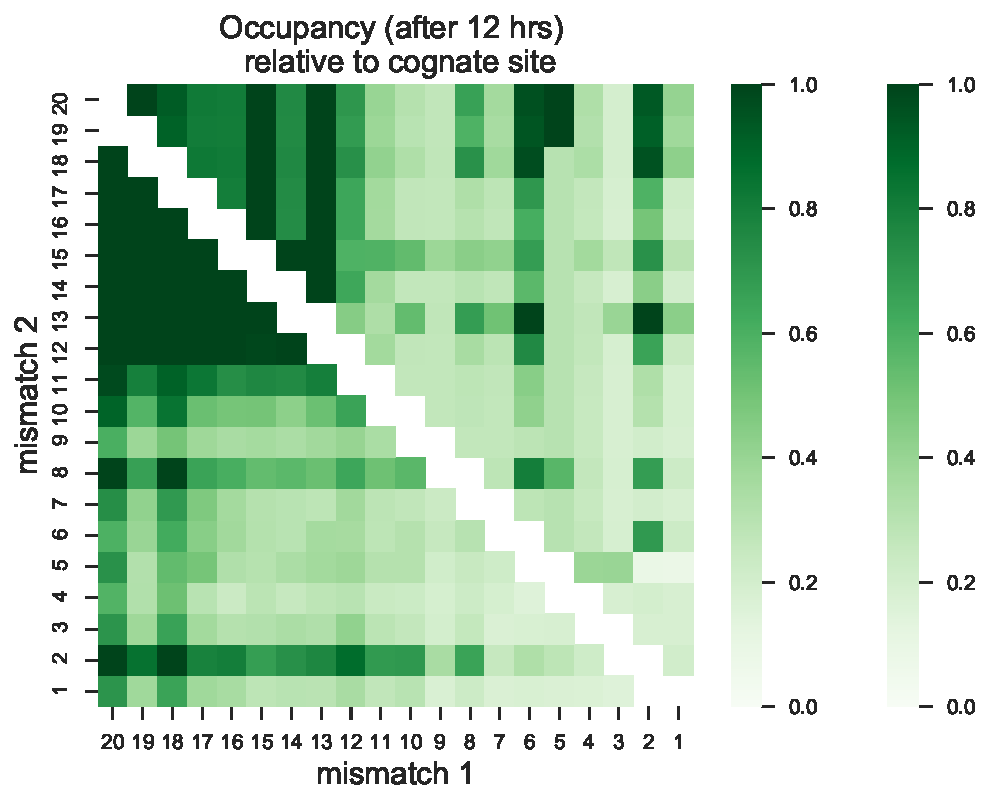
\includegraphics[scale=0.5]{fig20_10_10_2018.pdf}
\end{figure}


\begin{figure}[H]
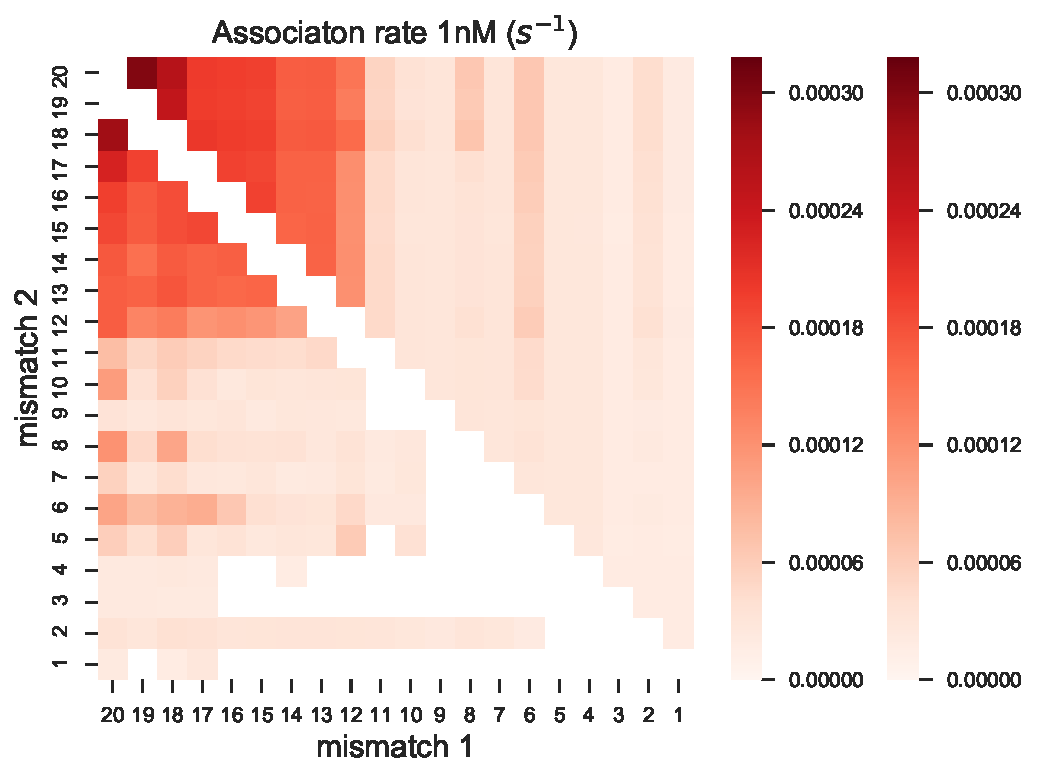
\includegraphics[scale=0.5]{fig21_10_10_2018.pdf}
\end{figure}

\begin{figure}[H]
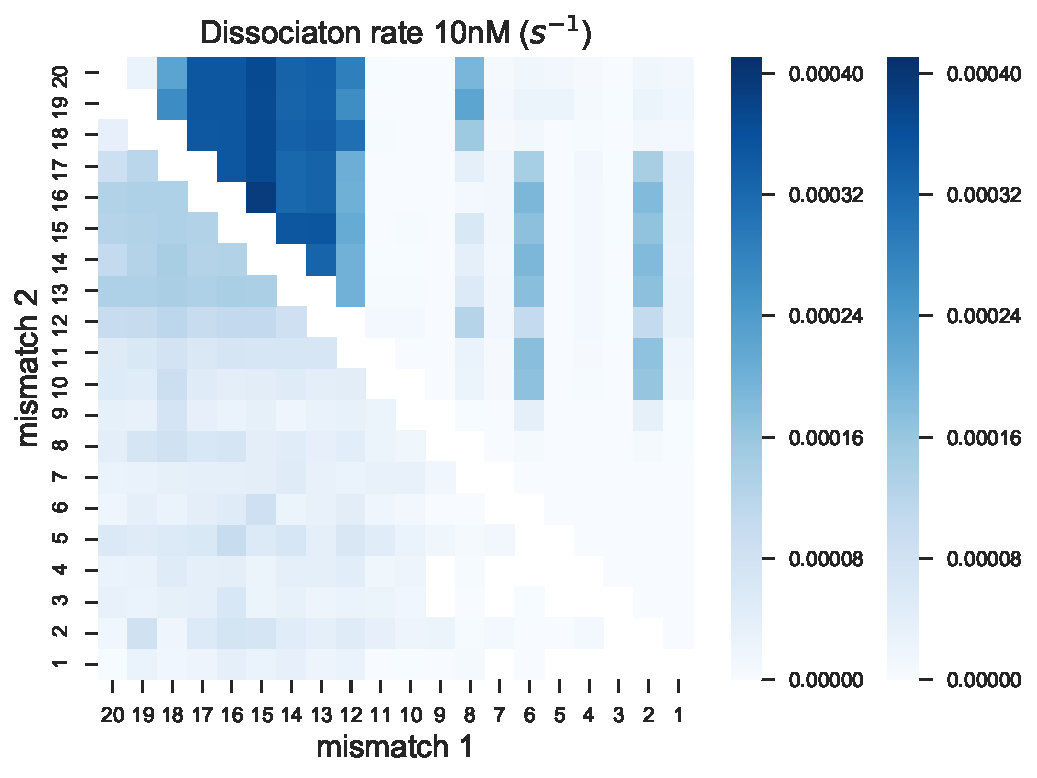
\includegraphics[scale=0.5]{fig22_10_10_2018.pdf}
\end{figure}


\section{predicting multiple mismatches}
We can predict the association rate for multiple mismatches. Note that these have not been provided as training.

\begin{figure}[H]
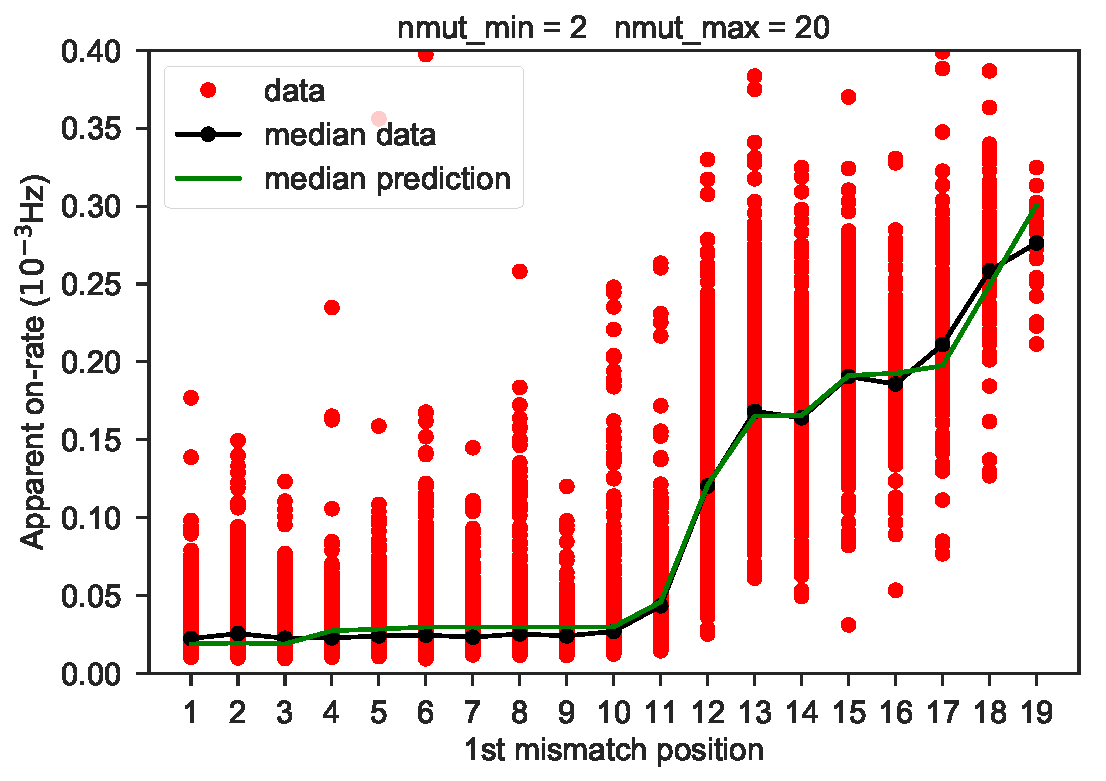
\includegraphics[scale=0.5]{fig31_10_10_2018.pdf}
\end{figure}


\section{Resulting Free-Energy landscape is consistent with Ilya's data}
\begin{itemize}
\item They assume equillibration and - using the Hill equation- estimate the dissociation constant. 
\item The log of this dissociation constant approximates the bound free-energy. This is the reason we have been plotting them as done in the previous sections.
\item This Aparant Binding Affinity (ABA) is then compared to the value of the cognate site. Hence, the on-target has free-energy - or $\Delta$ABA - of zero. 
\item Not used here, but we have a code in place that mimics his experiment and does not need to assume the system to be equillibrated. Indeed, when looking at his figures - even those published - the fit to the Hill Equation is not impressive. A more accurate $K_D$ estimate can be obtained by solving for the occupation after 10 minutes (the time at which they took their data).
\item One particularly nice experiment for us is where they analized targets with blocks of mismatches. Due to their high-throughput measurements, they have data for blocks of all lengths and starting positions. 
\item Interestingly, also Ilya's data shows that placing more than 2 mismatches does not further destabilize the system significantly. Again hinting towards 'class II'.
\item the figure superimposes the free-energy landscape obtained from Simulated Annealing - only using  Boyle's association data - and Ilya's experimental estimate of the same. 
\item \textbf{Conclusion: Without any imput from Ilya's data - no parameter estimation - we actually nearly manage to reproduce his signal based on Boyle's data.}
\end{itemize}


\begin{figure}[H]
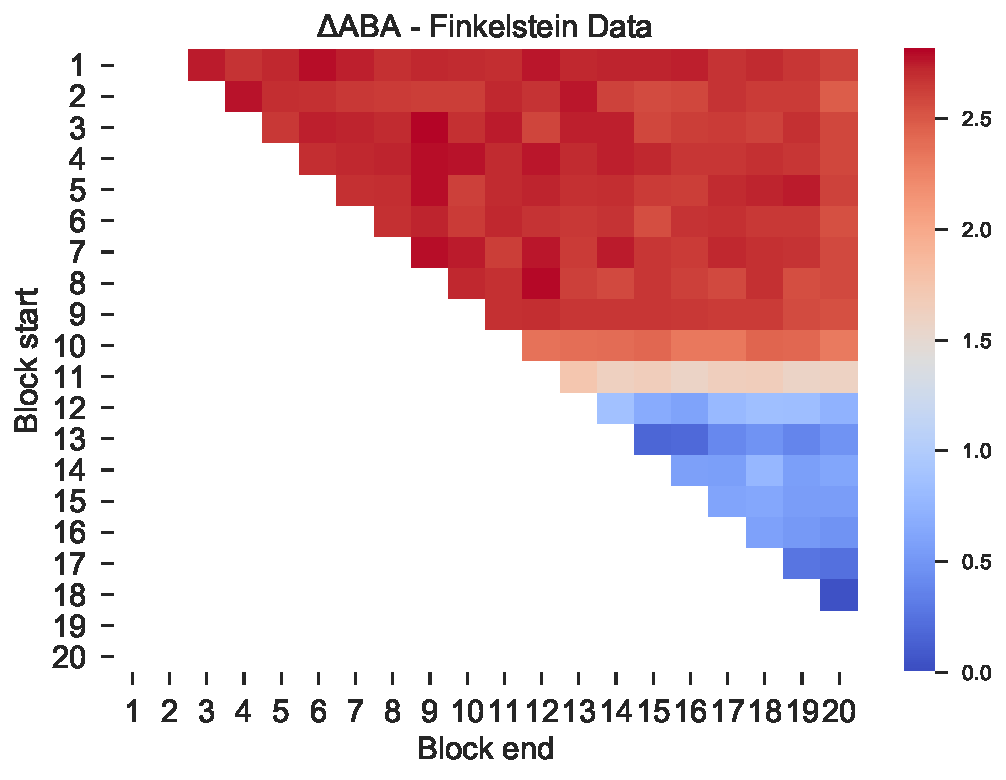
\includegraphics[scale=0.5]{fig41_10_10_2018.pdf}
\end{figure}

\begin{figure}[H]
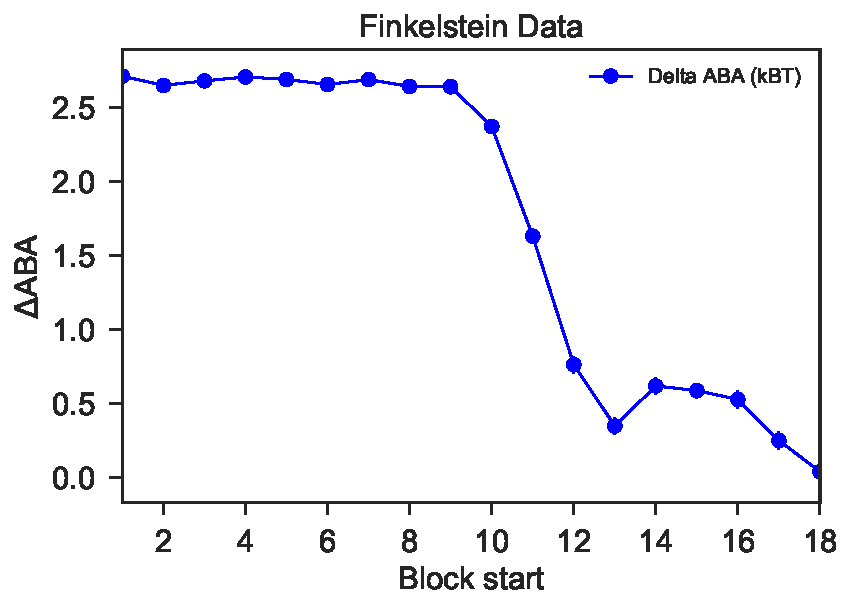
\includegraphics[scale=0.5]{fig42_10_10_2018.pdf}
\end{figure}

\end{document}